\documentclass[conference]{IEEEtran}
\IEEEoverridecommandlockouts
% The preceding line is only needed to identify funding in the first footnote. If that is unneeded, please comment it out.
\usepackage{cite}
\usepackage{amsmath,amssymb,amsfonts}
\usepackage{algorithmic}
\usepackage{graphicx}
\usepackage{textcomp}
\usepackage{xcolor}

\def\BibTeX{{\rm B\kern-.05em{\sc i\kern-.025em b}\kern-.08em
    T\kern-.1667em\lower.7ex\hbox{E}\kern-.125emX}}
\begin{document}

\title{YOLOv8n based Traffic Detection\\ }

\makeatletter
\newcommand{\linebreakand}{%
  \end{@IEEEauthorhalign}
  \hfill\mbox{}\par
  \mbox{}\hfill\begin{@IEEEauthorhalign}
}
\makeatother

\def\Affiliation{ School of Electrical Engineering }
\def\Organization{Telkom University, Indonesia}
\def\CityCountry{Bandung, Indonesia}

\author{\IEEEauthorblockN{Aura Syafa Aprillia Radim}
\IEEEauthorblockA{\textit{\Affiliation} \\
\textit{\Organization}\\
\CityCountry\\
syafaaura@student.telkomuniversity.ac.id }
\and
\IEEEauthorblockN{Muchammad 'Irfan Chanif Rusydi}
\IEEEauthorblockA{\textit{\Affiliation} \\
\textit{\Organization}\\
\CityCountry \\
chanifrusydi@student.telkomuniversity.ac.id}
\and
\IEEEauthorblockN{Surya Michrandi Nasution}
\IEEEauthorblockA{\textit{\Affiliation} \\
\textit{\Organization}\\
\CityCountry \\
michrandi@telkomuniversity.ac.id}
\linebreakand
% \IEEEauthorblockN{4\textsuperscript{th} Given Name Surname}
% \IEEEauthorblockA{\textit{dept. name of organization (of Aff.)} \\
% \textit{name of organization (of Aff.)}\\
% City, Country \\
% email address or ORCID}
% \and
\IEEEauthorblockN{Casi Setianingsih}
\IEEEauthorblockA{\textit{\Affiliation} \\
\textit{\Organization}\\
\CityCountry\\
setiacasie@telkomuniversity.ac.id}
% \and
% \IEEEauthorblockN{6\textsuperscript{th} Given Name Surname}
% \IEEEauthorblockA{\textit{dept. name of organization (of Aff.)} \\
% \textit{name of organization (of Aff.)}\\
% City, Country \\
% email address or ORCID}
}

\maketitle

\begin{abstract}
Dashcam is a camera placed on the dashboard of a vehicle. This device function is to capture footage of all events in front of the vehicle.
Security and safety have become a significant concern in various sectors, including transportation and public roads. 
Traffic accidents caused by drivers' ignorance of objects around the vehicle are still a severe problem on the highway
In this study, a simple dashcam built from an edge computer was developed by combining a camera placed on the center of the vehicle dashboard and object detection algorithms.   
Next, object detection is carried out on the images that have been collected. The object detection system approach is carried out using YOLOv8, which is the latest variant of the YOLO series.
This research is expected to be one step in the development of an Intelligent Transportation System that is in accordance with traffic conditions in Indonesia.
The results obtained by testing the system in a real-world environment show that the system can detect traffic objects in real time.
The best result of 15 frames per second in the traffic object detection inference process is achieved when the edge computer uses 10 watts of power.
\end{abstract}

\begin{IEEEkeywords}
object detection,You Only Look Once, YOLOv8, dashcam, ADAS
\end{IEEEkeywords}

\section{Introduction}
% bahas dashcam, YOLO 8, sekarang ini banyak yang memakai dashcam, tapi dashcam yang ada sekarang hanya untuk merekam, belum ada yang bisa mendeteksi objek di depannya
Security and safety have become a significant concern in various sectors, including transportation and public security. 
On the highway, traffic accidents caused by drivers' ignorance of objects around the vehicle are still serious problems. Intelligent and effective object detection technology is becoming increasingly important in monitoring ahead and approaching traffic\cite{b1}.

A dashboard camera (Dashcam) is placed on a vehicle's dashboard. This device usually serves to record all events in front of the vehicle. Dashcam is one of the devices that the demand proliferates in the market. Currently, a dashcam serves as a device to record events in front of the vehicle, and then the recording is used as evidence of an accident or proof of insurance claims. However, dashcams could also be used for other purposes, such as one of the components of an Autonomous Driving Assistance System (ADAS). 

In this paper, we propose a simple solution to prevent accidents among vehicles. 
Our solution is by implementing object detection and Single Board Computer (SBC) as processing unit. 
Objects in front of the camera can be detected by Convolutional Neural Network. 

%  carikan paper mengenai penembangan dashcam
The content of this paper is organized as follows. Section 2 presents the literature review. Section 3 presents the system design. Section 4 presents experimentation in the process of developing the system. Section 5 presents the conclusion and future work.

\section{Literature Review}
\subsection{Dashcam}
% Masukin litarasi dashcam, terakhir masukin related work monocular raspbberry pi
Dashcam has been widely used by drivers to record traffic on the road. Many believe that dashcam is essential part of the vehicles.
There are several reasons to install a dashcam, including the insurance corporations favorable insurance rates for drivers and the collection of material that can be used as evidence in legal procedures. 

To such a degree that both Chinese and South Korean governments oblige public transportation and commercial vehicles to install a dashcam to assist in investigating traffic accidents\cite{Korea Dashcam}.
Despite the importance of being widely known, only some utilize dashcams for purposes other than recording the road and traffic conditions. In this paper, we implement object detection in a camera placed on a vehicle's dashboard along with the processing unit and display.
\subsection{Object Detection}
Object Detection is one of the essential tasks in the computer vision field, mainly dealing with detecting instances of visual objects and then categorizing them into several classes\cite{b2}.
With this kind of identification and localization, object detection can be used to count objects in a scene and determine and track their precise locations, all while accurately labeling them.
Object detection has been widely used for face detection, vehicle detection, pedestrian counting, web images, security systems, and driverless cars.
Object detection has undergone many changes and developments in the past twenty years. Although it is commonly divided into two periods: "traditional object detection" and "deep learning based".
In 2012, Krizhevsky et al.~\cite{b3} proposed a deep convolutional network trained on a subset of ImageNet. 

This network, called AlexNet, was the forerunner of the YOLO model.
A year later, Girshick et al. \@ proposed a new object detection framework called R-CNN~\cite{b3} because it combined region proposals with CNNs to detect objects in images.
Since then, the object detection research and development field has been rapidly advancing, with new models, datasets, and techniques emerging rapidly. 

%tambahkan gambar atau ilustrasi CNN atau YOLO 
With the birth of AlexNet, the YOLO (You Only Look Once) model was introduced in 2015. 
The original base YOLO model can achieve 45 frames per second. The smaller version, Fast YOLO, can achieve 155 frames per second. YOLO outperforms DPM and R-CNN on the Picasso Dataset and People-Art Dataset~\cite{You Only Look Once}.

In the early period of making this paper, YOLOv7 was the latest version of YOLO. 
However, as of January 2023, YOLOv8 was introduced by Ultralytics, the same software company that released YOLOv3 and YOLOv5. In the early period of making this paper, YOLOv7 was the latest version of YOLO. 
However, as of January 2023, YOLOv8 was introduced by Ultralytics, the same software company that released YOLOv3 and YOLOv5. 
As of now, YOLOv8 is one of the latest State of The Art (SOTA) open-source object detection models. 
Following its predecessor, YOLOv8 offers several model sizes. 
From the YOLOv8n as the smallest model, YOLOv8l as the medium model, and YOLOv8x as the largest model. 
YOLOv8n was chosen as the model due to its small size and compatibility with edge computing devices. YOLOv8n used 168 layers with over 3 million parameters with a computation cost of around 8 GFLOPs

\subsection{COCO Dataset}\label{AA}
The COCO dataset is a large-scale object detection, segmentation, and keypoint dataset. In total, The Microsoft Common Objects in COntext contains 91 common object categories, with 82 of them having more than 5,000 labeled instances~\cite{COCO Dataset}.
The first release of the COCO Dataset was in 2014. In 2014, the COCO Dataset had 83,000 images in the  train split, and 41,000 images in the validation split.
After taking community feedback, the COCO Dataset increases the total number of images and changes its split proportion. In the 2017 release, the train2017 split had 118,000 image files and 5,000 images in the val2017 split.
Given its size, COCO Dataset is widely used by State of the Art Object Detection Model to train and evaluate the model performance.

Despite its popularity, the COCO Dataset has some drawbacks. 
Although the COCO Dataset contains quite a large number of image classes, it has an imbalanced class distribution 
For example, as shown in Fig.\ref{fig:original_coco_classes_count} the total number of annotated objects for person class is 64115, while the hair dryer class is only around 100. Additionally, for this research, the model doesnt need to detect anything other than objects that relate to traffic.
\begin{figure}[!h]
\centering
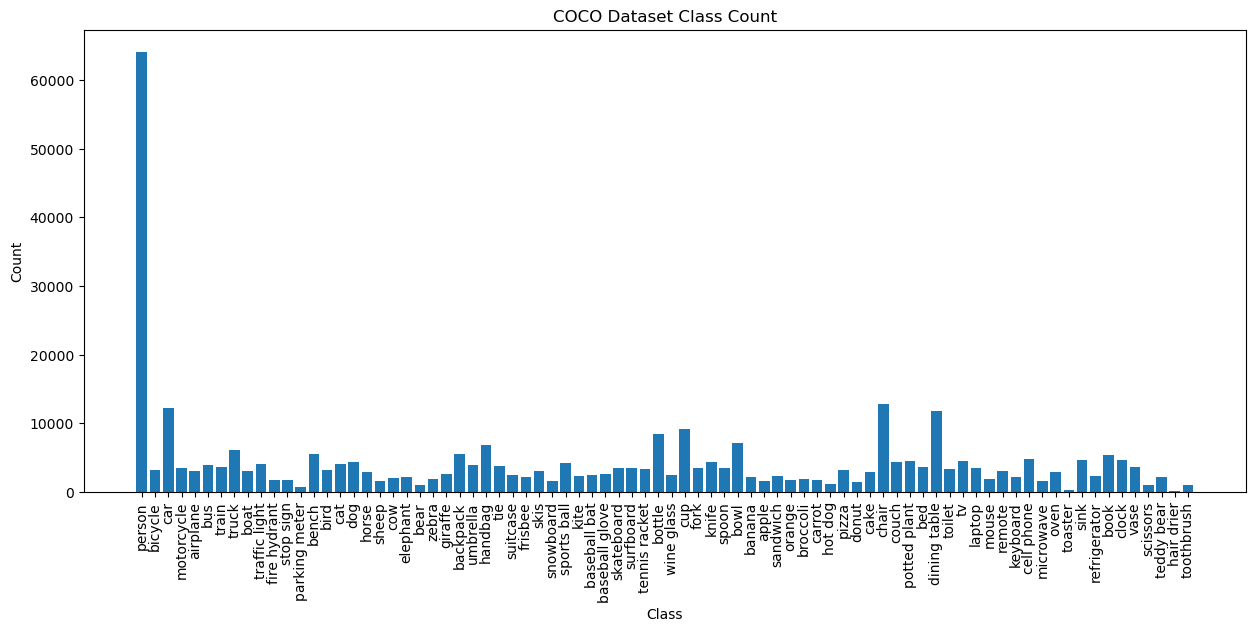
\includegraphics[width=0.5\textwidth,keepaspectratio]{coco_class_count.png}\label{fig:original_coco_classes_count}
\caption{COCO Dataset Class Count}
\end{figure}


\subsection{Enhancing the Dataset}\label{Filtering}
As mentioned earlier, COCO dataset contains 80 classes. Traffic-related object classes are all that is needed in this research.
Therefore, we filtered the dataset to only contain 12 classes. The classes are:
Car Truck Bus Motorcycle Bicycle Traffic Light Stop Sign Train Hydrant Cat Dog
The result is 78,663 images in training split with 12 classes. This amount of data was reduced from 122,125 images in original dataset. The training time of our model is expected to be reduced by decreasing the size of the dataset.
\begin{figure}[h!]
\centering
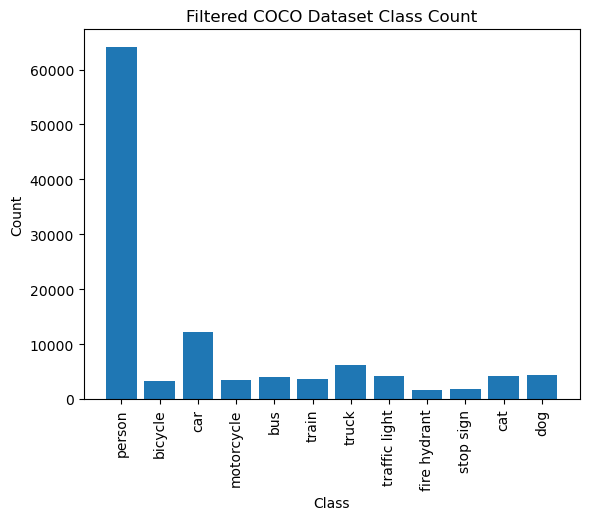
\includegraphics[width=0.4\textwidth]{filtered_coco_class_count.png}
\caption{Filtered COCO Dataset Class Count}
\label{fig:COCOFiltered}
\end{figure}

\begin{figure}[h!]
\centering
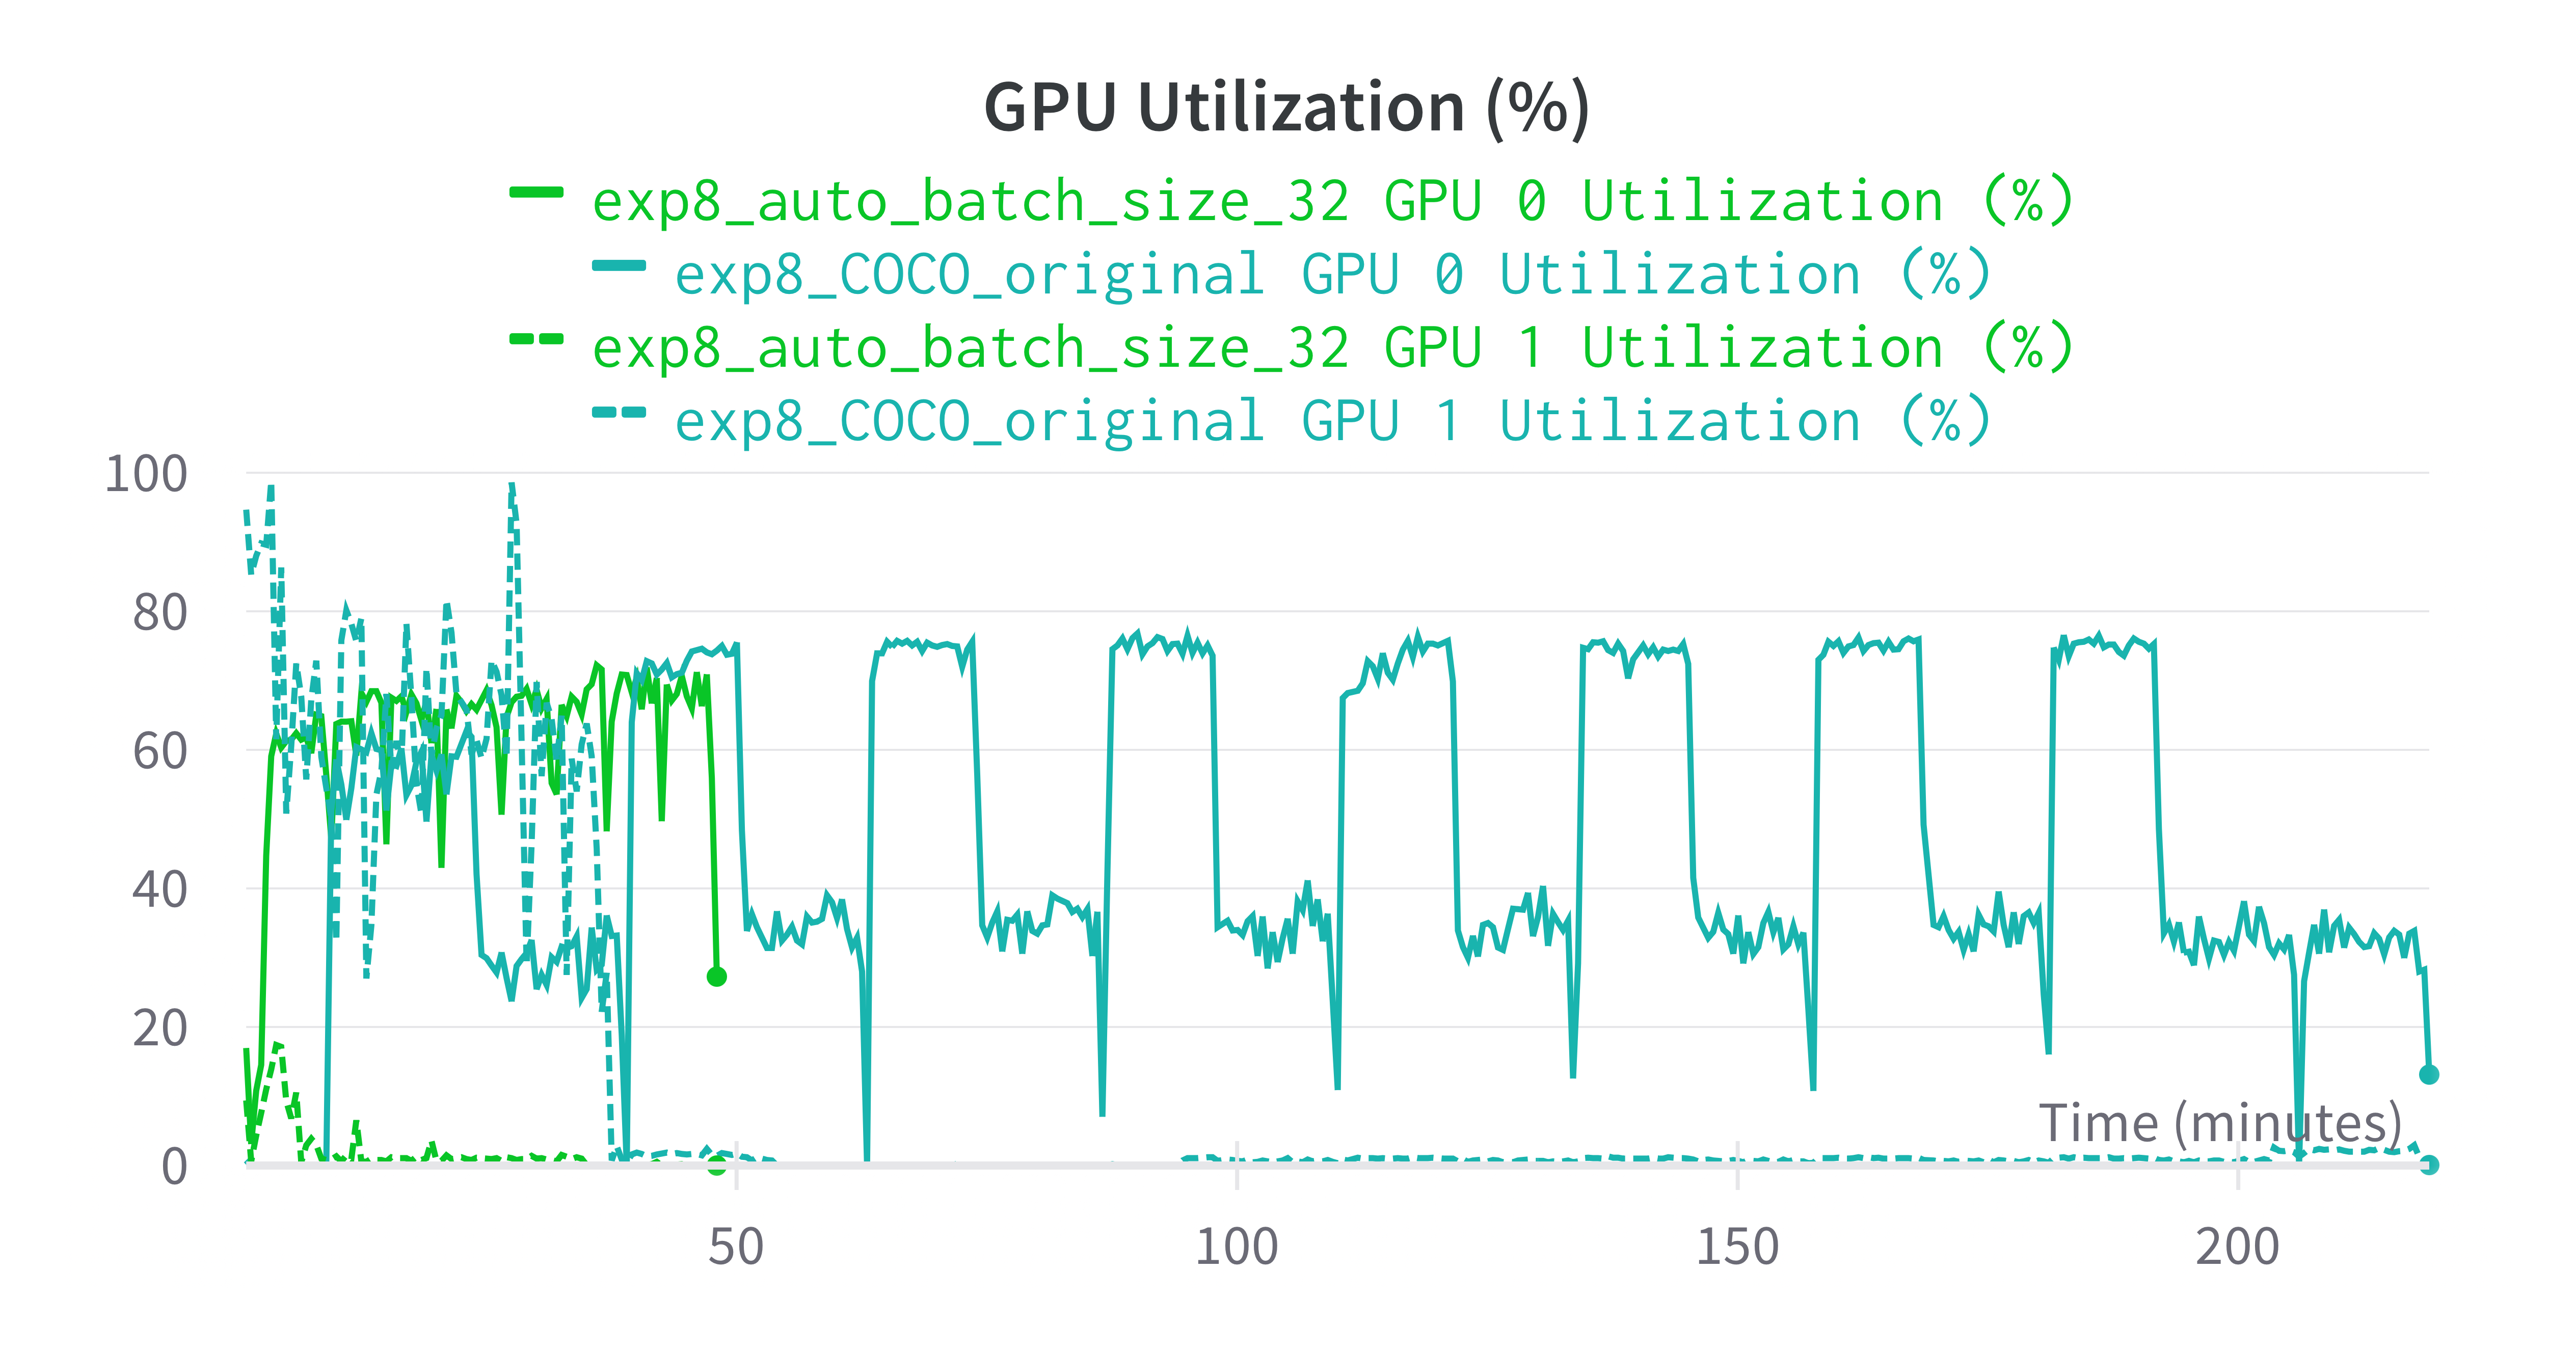
\includegraphics[width=0.4\textwidth,keepaspectratio]{gpu_utilization_comparison_original_and_filtered.png}
\caption{Comparison of GPU Utilization between training the model using filtered dataset and original dataset}
\label{fig:original_filtered_gpu_utilization}
\end{figure}

\begin{figure}[h!]
\centering
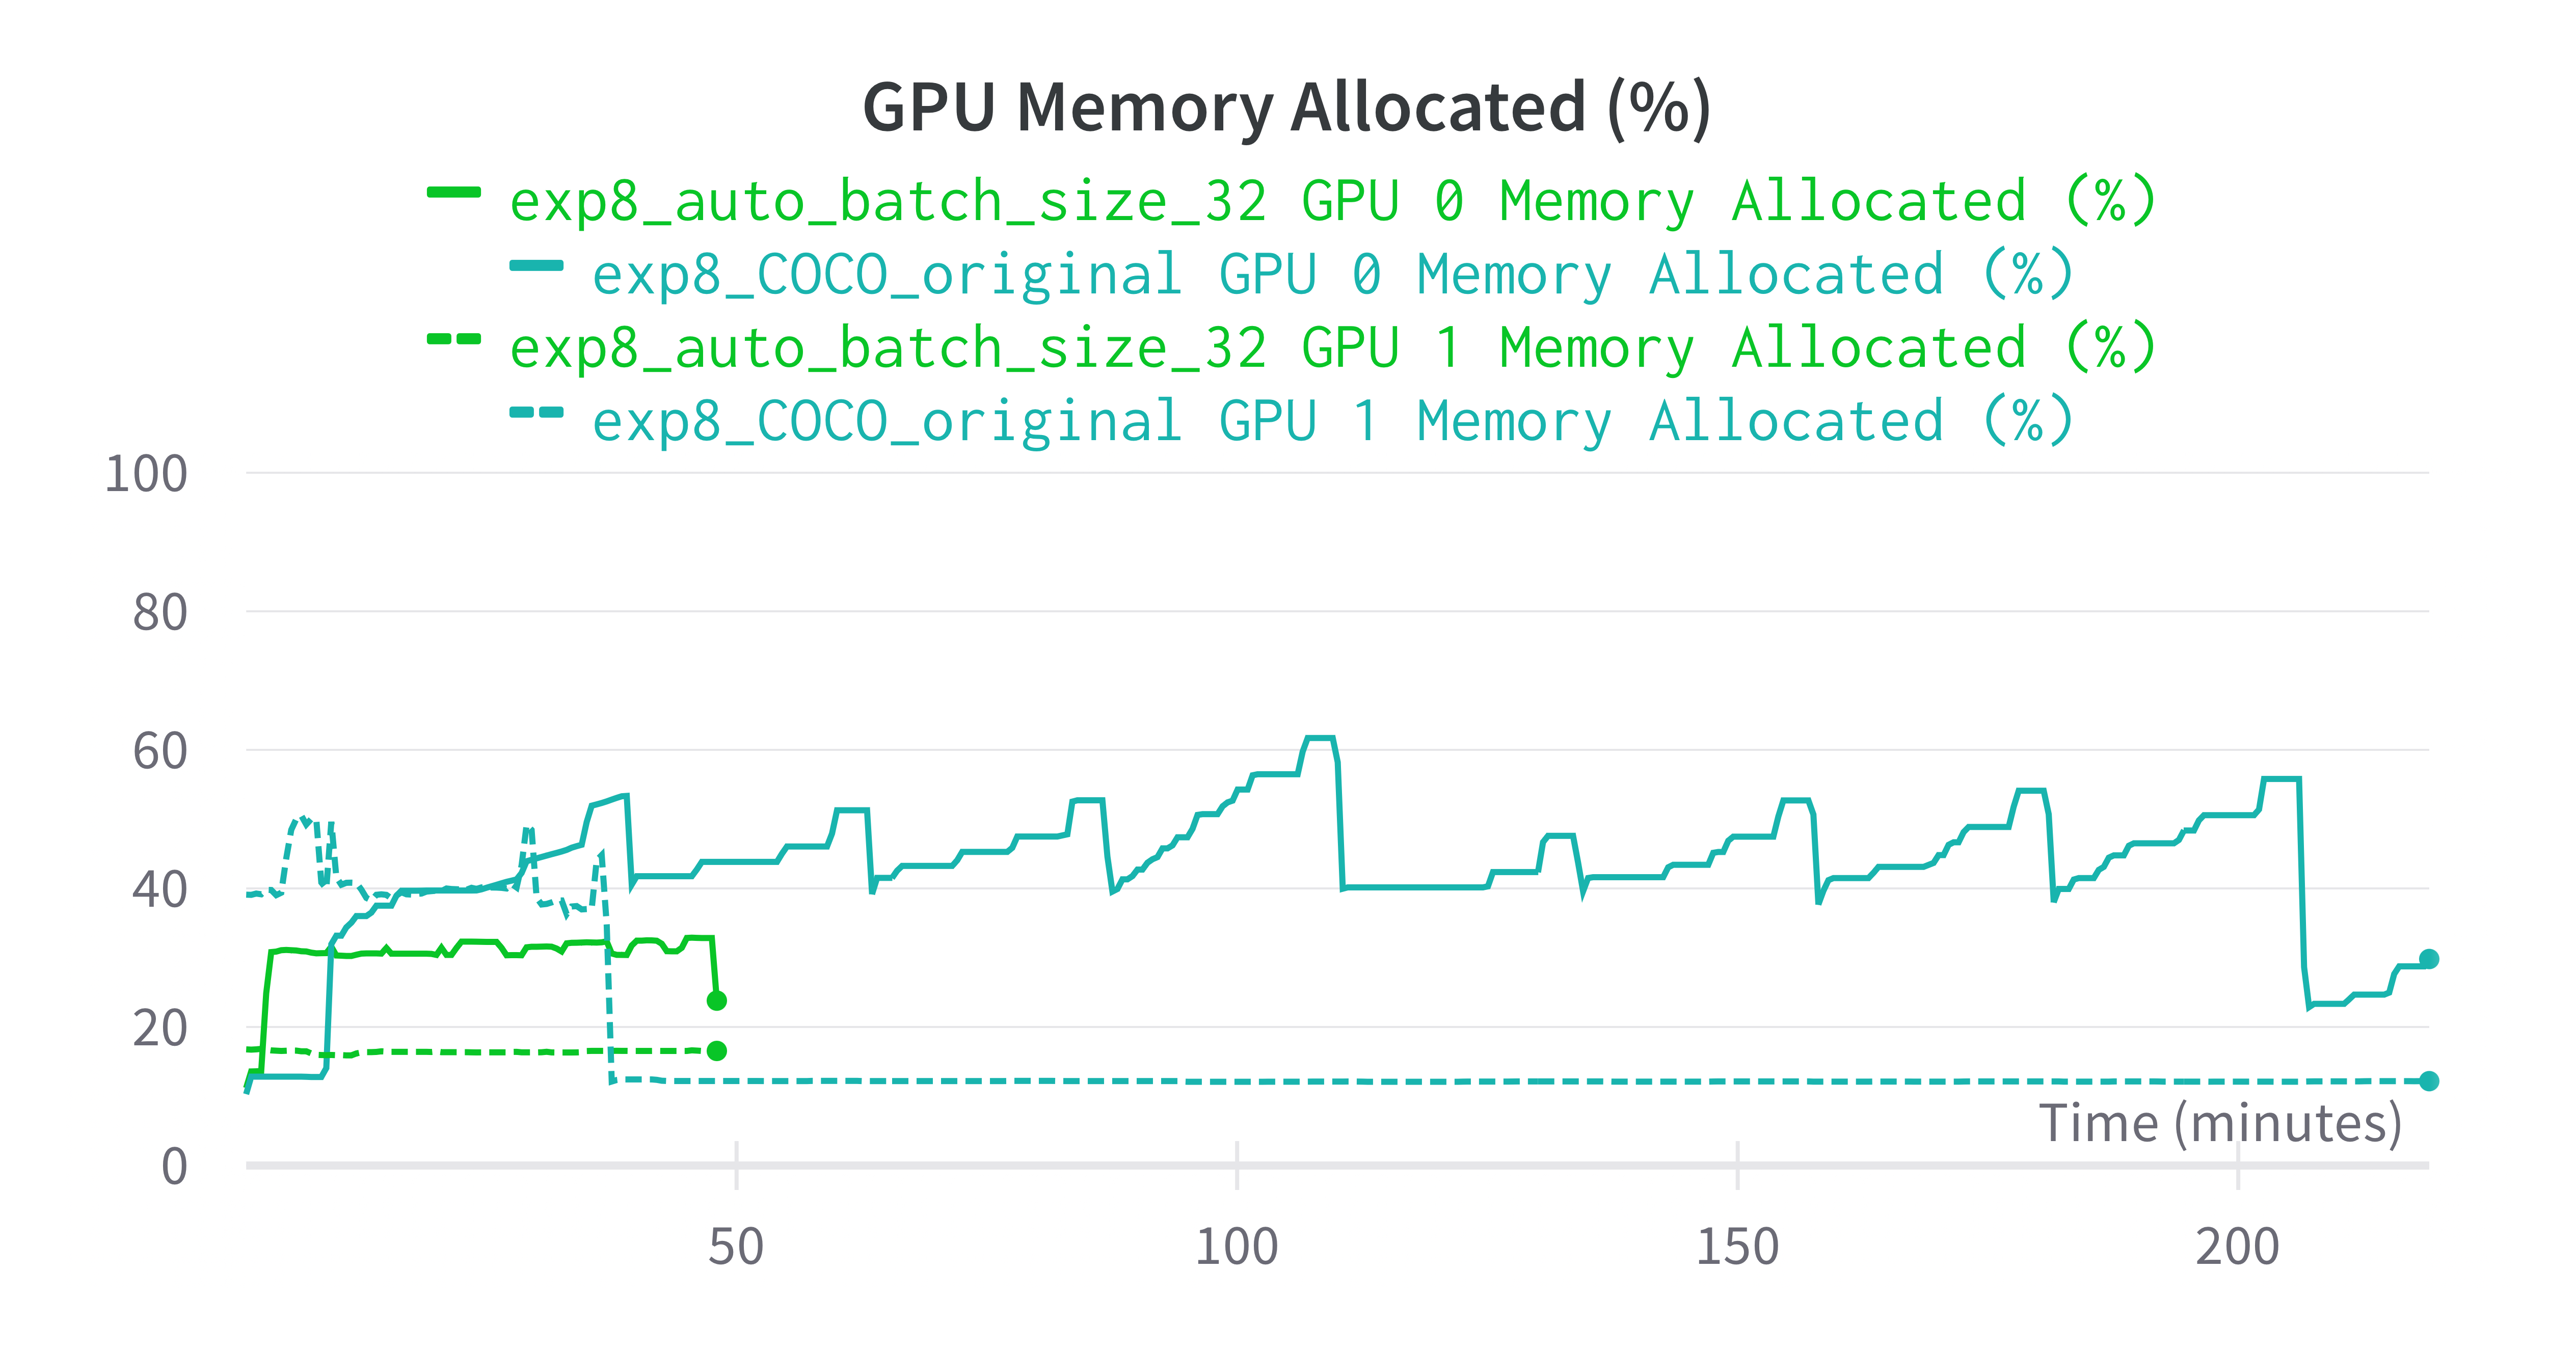
\includegraphics[width=0.3\textwidth,keepaspectratio]{memory_utilization_comparison_original_and_filtered.png}
\caption{Comparison of GPU Memory Utilization between training the model using filtered dataset and original dataset}
\label{fig:original_filtered_memory_utilization}
\end{figure}
In addition, as shown in Fig. \ref{fig:original_filtered_gpu_utilization} and Fig.\ref{fig:original_filtered_memory_utilization}, the filtered dataset has lower GPU Utilization and Memory Utilization. This means that the filtered dataset is more efficient to train.
Thus allowing us to push model training further.
In terms of metrics results, the model trained using a filtered dataset showed a better result, Fig.~\ref{fig:training_comparison}. The model trained on a filtered dataset with eight epochs reached mAP.95 of 0.298. While the one trained with the original train2017 split only reached 0.135.
\begin{figure}
\centering
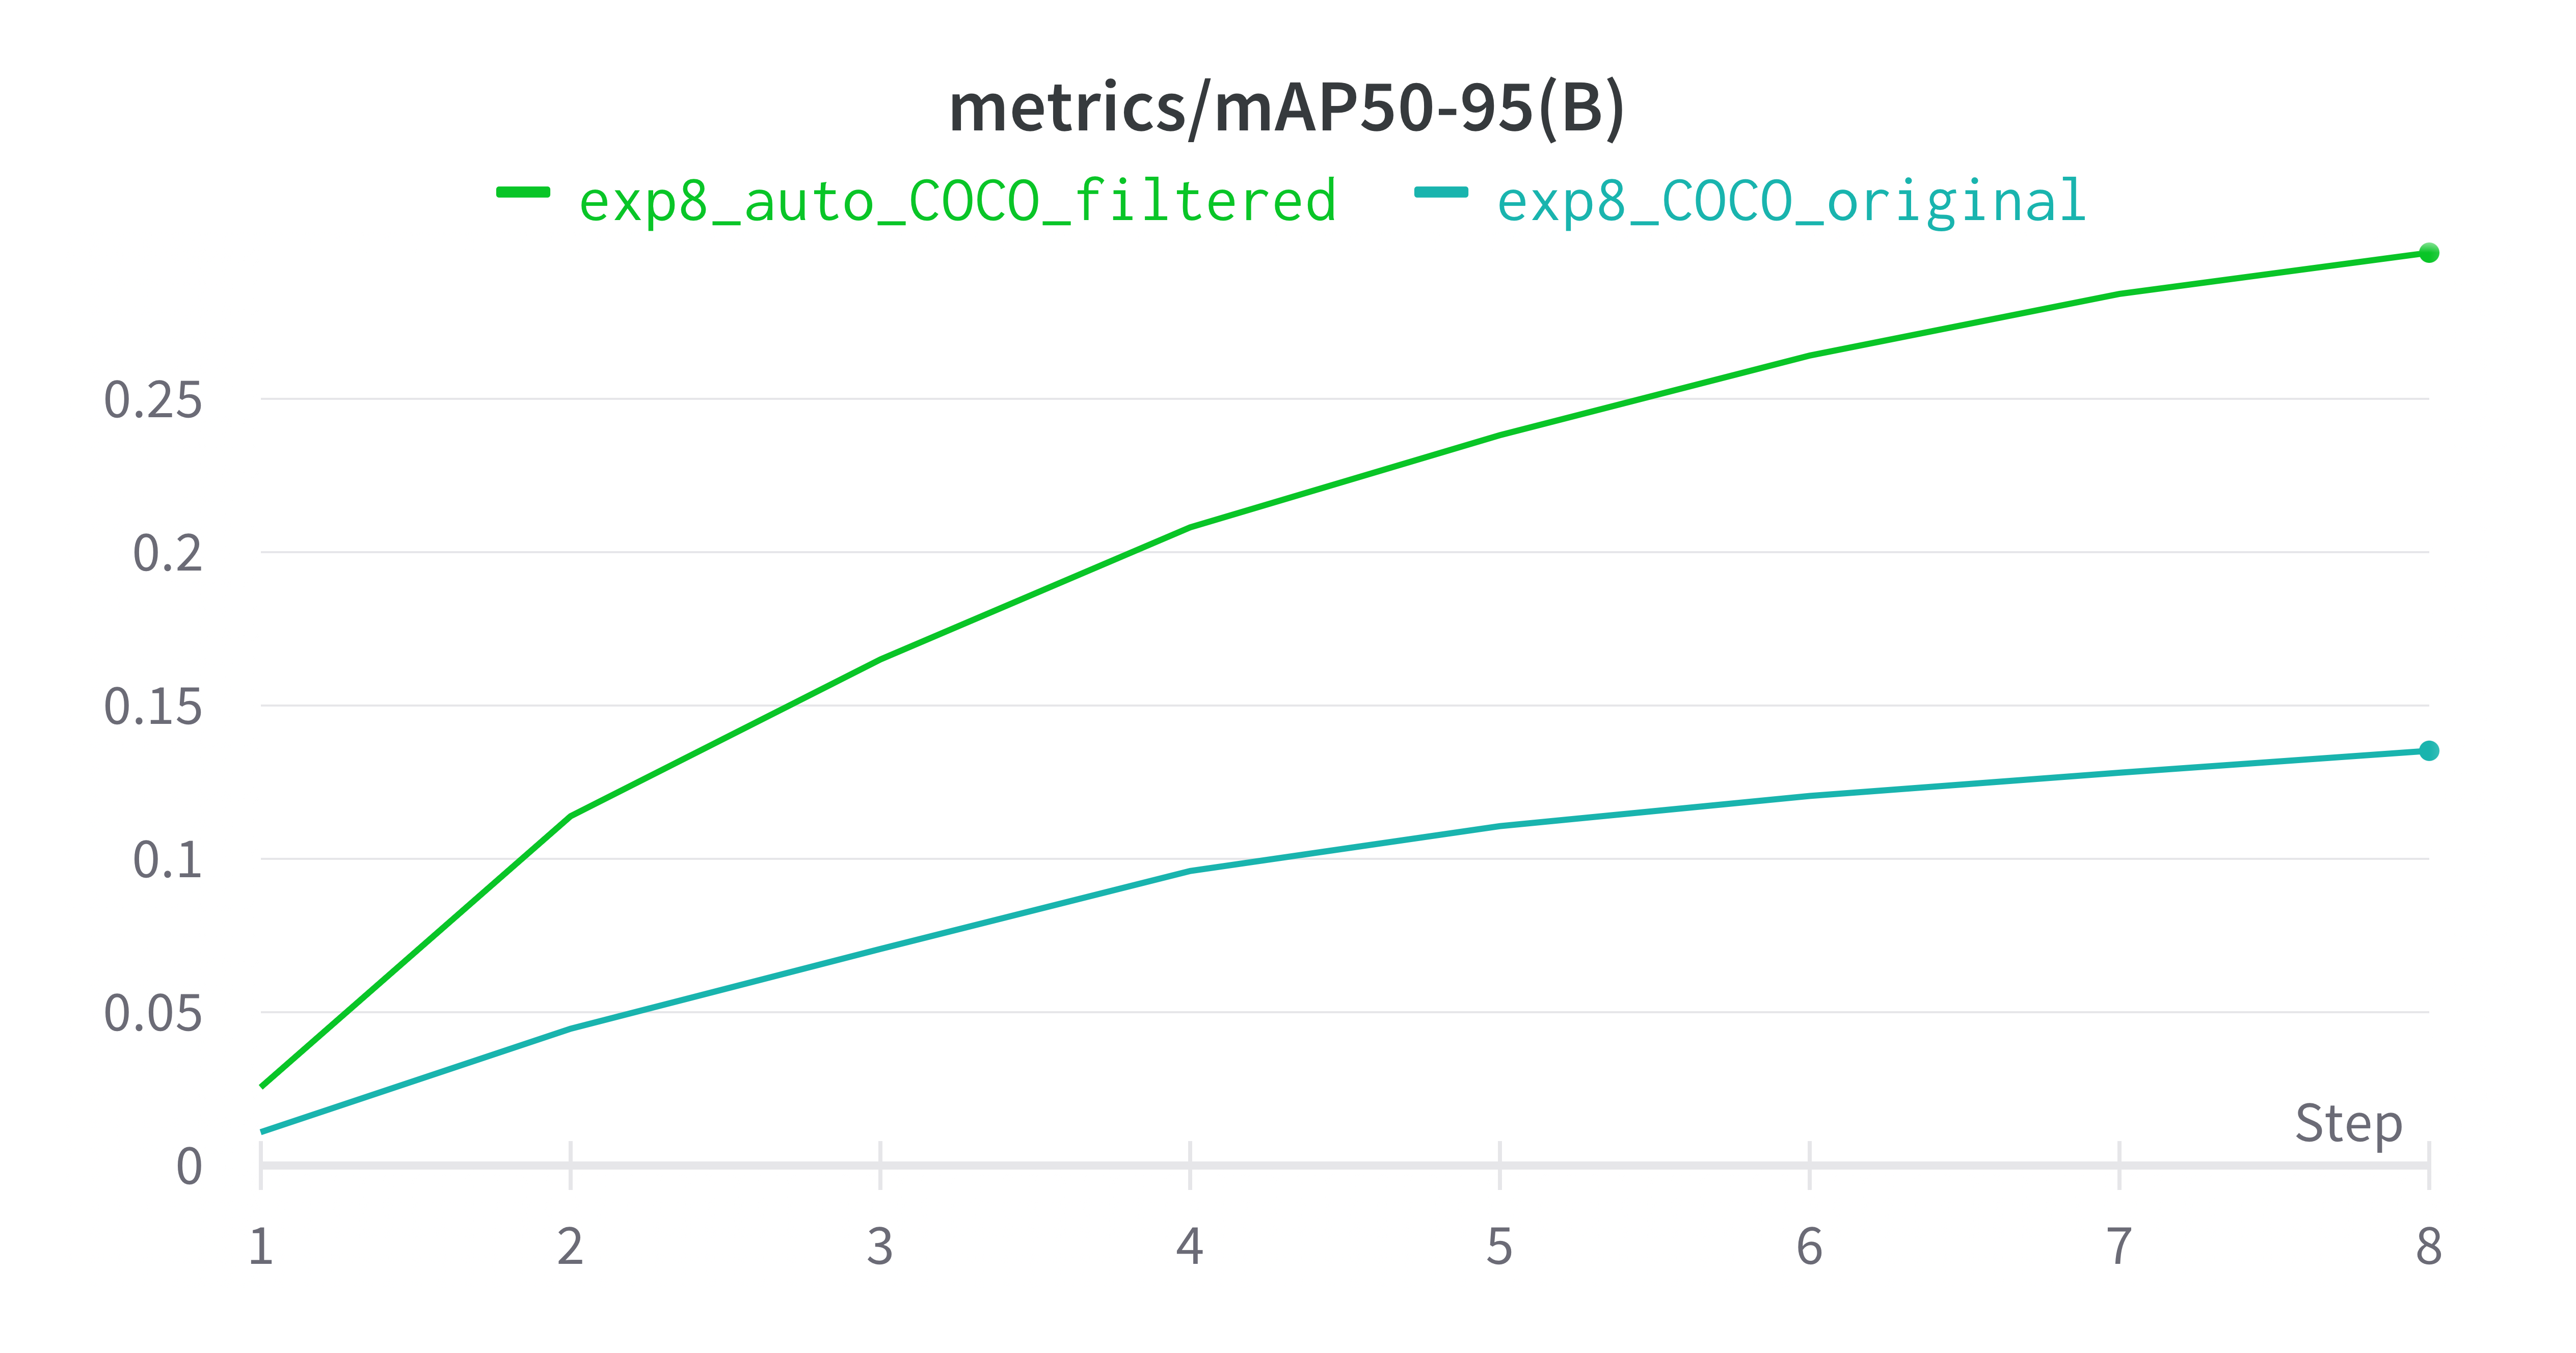
\includegraphics[width=0.4\textwidth,keepaspectratio]{comparison_mAP_filtered.png}
\caption{Comparison of mAP50-95 between training the model using filtered dataset and original dataset}
\label{fig:training_comparison}
\end{figure}

\subsection{Performance Metrics}
For training and validation purposes, we focus on mAP (mean Average Precision), Precision, and recall. mAP is the average of AP (Average Precision) over all classes. AP is the area under the precision-recall curve.
We compare mAP averaged for IoU (Intersection over Union) thresholds from .50 to .95 with .05 increments (MS COCO standard metric, abbreviated as mAP50-95) and mAP50 (PASCAL VOC metric, abbreviated as mAP50) \cite{COCO Dataset}. 
Precision and Recall in  this experiment is a relative measure because it depends on the threshold value.
Precision is calculated by dividing the True Positive by the sum of True Positive and False Positive. 
Precision is calculated using \eqref{equation1}.
\begin{equation}
Precision = \frac{TP}{TP+FP}
\label{equation1}
\end{equation}
Recall calculated by dividing True Positive by the sum of True Positive and False Negative.
\begin{equation}
Recall = \frac{True Positive}{TruePositive+FalseNegative}
\end{equation}
The threshold value determines whether the prediction is Positive or Negative. For example, if the threshold is 0.5, then the prediction is positive if the IoU is greater than 0.5. Otherwise, the prediction is negative.

Both Precision and Recall are relative to the threshold value and are usually used in the form of Precision-Recall Curve. We can calculate the area under the curve to get the Average Precision
To get the mAP value, we need to calculate the Average Precision for each class.
\begin{equation}
mAP = \frac{1}{n}\sum_{i=1}^{n}AP_i
\label{mAP}
\end{equation}
$\eta$ is the number of classes.
This is the main reason filtering Dataset would be beneficial in the training process. As we use a filtered dataset, the value of $\eta$ in equation ~\ref{mAP} is 12 instead of 80.


\section{System Design}
% Flowchart di sini aja
% Fig 1 ceritakan lebih detail
% cerita singkat kita implementasi di jetson nano]
\subsection{Related Work}
Nasution et al.\cite{Road Information Collector} proposed a system that can detect vehicles and street lanes. The image feed was captured using a smartphone and then processed using the ImageAI library with RetinaNet for COCO as an object detection modelproposed a system that can detect vehicles and street lanes. The image feed was captured using a smartphone and then processed using the ImageAI library with RetinaNet for COCO as an object detection model


Nasution \& Dirgantara, 2023, proposed pedestrian detections for Autonomous Driving Assistance System (ADAS) using YOLOv5 and Raspberry Pi 4 as the edge computer. The pedestrian detection system is only capable of delivering 0,9 frames per second [6].

\subsection{System Overview}
In this section, we will discuss the system overview. The system consists of 3 main hardware components. 
The first component is the camera. The camera is used to capture the image.
The second component is the edge computer. The edge computer is used to process the image. 
The third component is the display. The display is used to show the result of the image processing.
\begin{figure}[!ht]
\centering
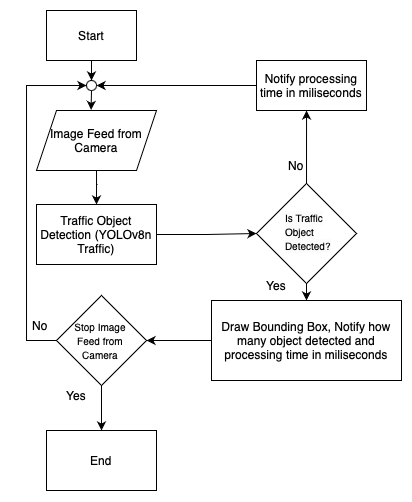
\includegraphics[width=0.4\textwidth,keepaspectratio]{Proposed Flowchart.png}
\caption{Proposed Flowchart of the system}
\label{fig:flowchart}
\end{figure}


Fig.\ref{fig:flowchart} shows the flowchart of proposed method of detecting traffic objects. First, the camera captures the image frame by frame, followed by preprocessing the images before feeding them to the YOLO model. The YOLO model provides the bounding point coordinates and probability for each class for all detected objects. The bounding box and class are then drawn on the image. The image with the bounding box and class is then displayed on the screen.

\subsection{Edge Processing Unit}
As Nasution and Dirgantara (2023) used Raspberry Pi 4 as their processing unit and only managed to get 0.9 FPS, we decided to find a more robust edge computer that was similar in price. The availability of GPU is another factor that needs to be considered. Since GPU is a crucial component in deep learning, an edge computer with a GPU is preferred. Jetson Nano is powered by a Quad Core ARM-A57 CPU with 32 cores of Maxwell GPU. This Maxwell GPU is the main selling point of Jetson Nano because it has CUDA Core, allowing us to run an accelerated deep-learning model.used Raspberry Pi 4 as their processing unit and only managed to get 0.9 FPS, we decided to find a more robust edge computer that was similar in price. The availability of GPU is another factor that needs to be considered. Since GPU is a crucial component in deep learning, an edge computer with a GPU is preferred. Jetson Nano is powered by a Quad Core ARM-A57 CPU with 32 cores of Maxwell GPU. This Maxwell GPU is the main selling point of Jetson Nano because it has CUDA Core, allowing us to run an accelerated deep-learning model.

\subsection{Experimental Setup}
In this section, we will discuss  the experimental setup. We are using Pytorch as the deep learning framework in Python  3.
Model training was conducted on Geforce RTX 3090, 24 GB Video RAM, 32GB RAM, Intel Core i3-12100 4 Core 8 Thread, running on Windows 10
Model inference and testing was performed on Jetson Nano 4GB. The camera used in this experiment is Lifecam Studio by Microsoft.
Ubuntu 20.04.2 LTS on top of Jetpack 4.6 is being run on the Jetson Nano that we use. The Jetson Nano 4GB is chosen as the edge computer of choice due to its affordability as Jetson Nano is the cheapest edge computer in the Nvidia Jetson Series.
\subsection{Testing Dataset}
As mentioned earlier, we are using the COCO dataset to train and validate the model, especially train20117 and val2017. However, we filtered the dataset to only contain 12 classes. The classes are
Car, Truck, Bus, Motorcycle, Bicycle, Traffic Light, Stop Sign, Train, Hydrant, Cat, Dog. The result is 78000 images with 12 classes.
For inference and real-world testing, we gather our own data by recording traffic conditions in Bandung, Indonesia. The data was recorded using the camera mentioned earlier.
As some part of the traffic footage that we collected, we also utilized it as an addition to the training dataset. This is because Indonesia's traffic condition is different from other countries. In Indonesia, a motorcycle is more often used than a car.
If we refer to the filtered COCO dataset in Fig.\ref{fig:COCOFiltered}, the number of motorcycle is lower than the number of car class. Therefore, we need to add more motorcycle data to the dataset.
\begin{figure}[h]
\centering
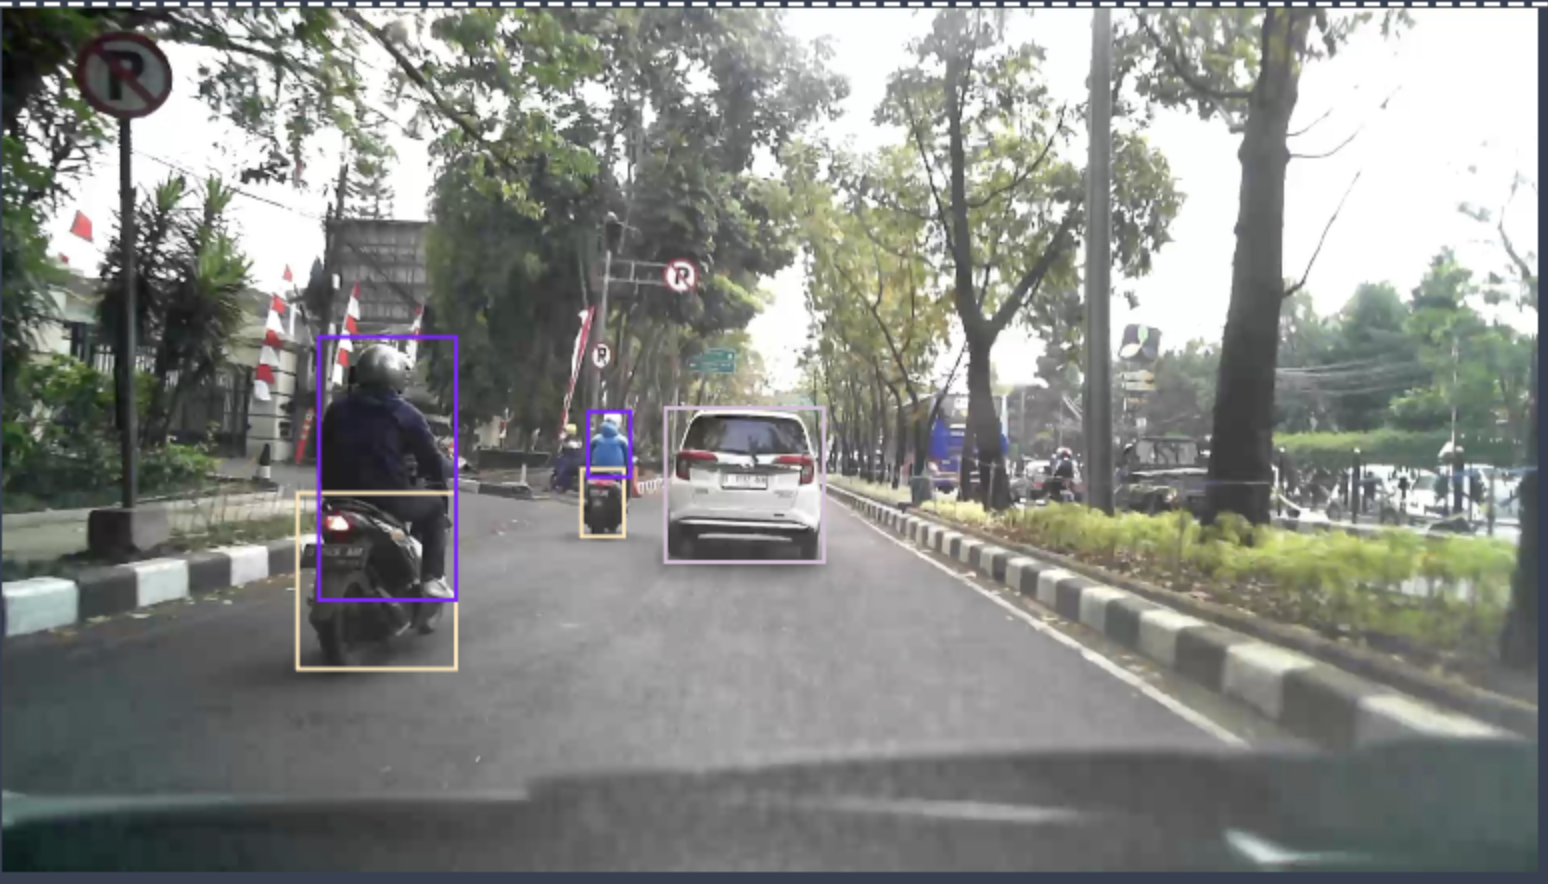
\includegraphics[width=0.4\textwidth,keepaspectratio]{sample_dataset.png}
\caption{Sample of annotated image from footage that we collected}
\end{figure}

\subsection{Training}
Before we begin our YOLOv8n-Traffic model training with high epochs, we want to find the optimal hyperparameter configuration for our use case. We conducted various training configurations with 8 epochs to save time. Although each run for one configuration is only 8 epochs, it still takes about 1 to 2 hours. The result can be obtained faster than training with 100 epochs for each configuration.
Different batch sizes, learning rates, and optimizers were used. Batch sizes 16 and 32 were chosen.
\begin{figure}[h]
\centering
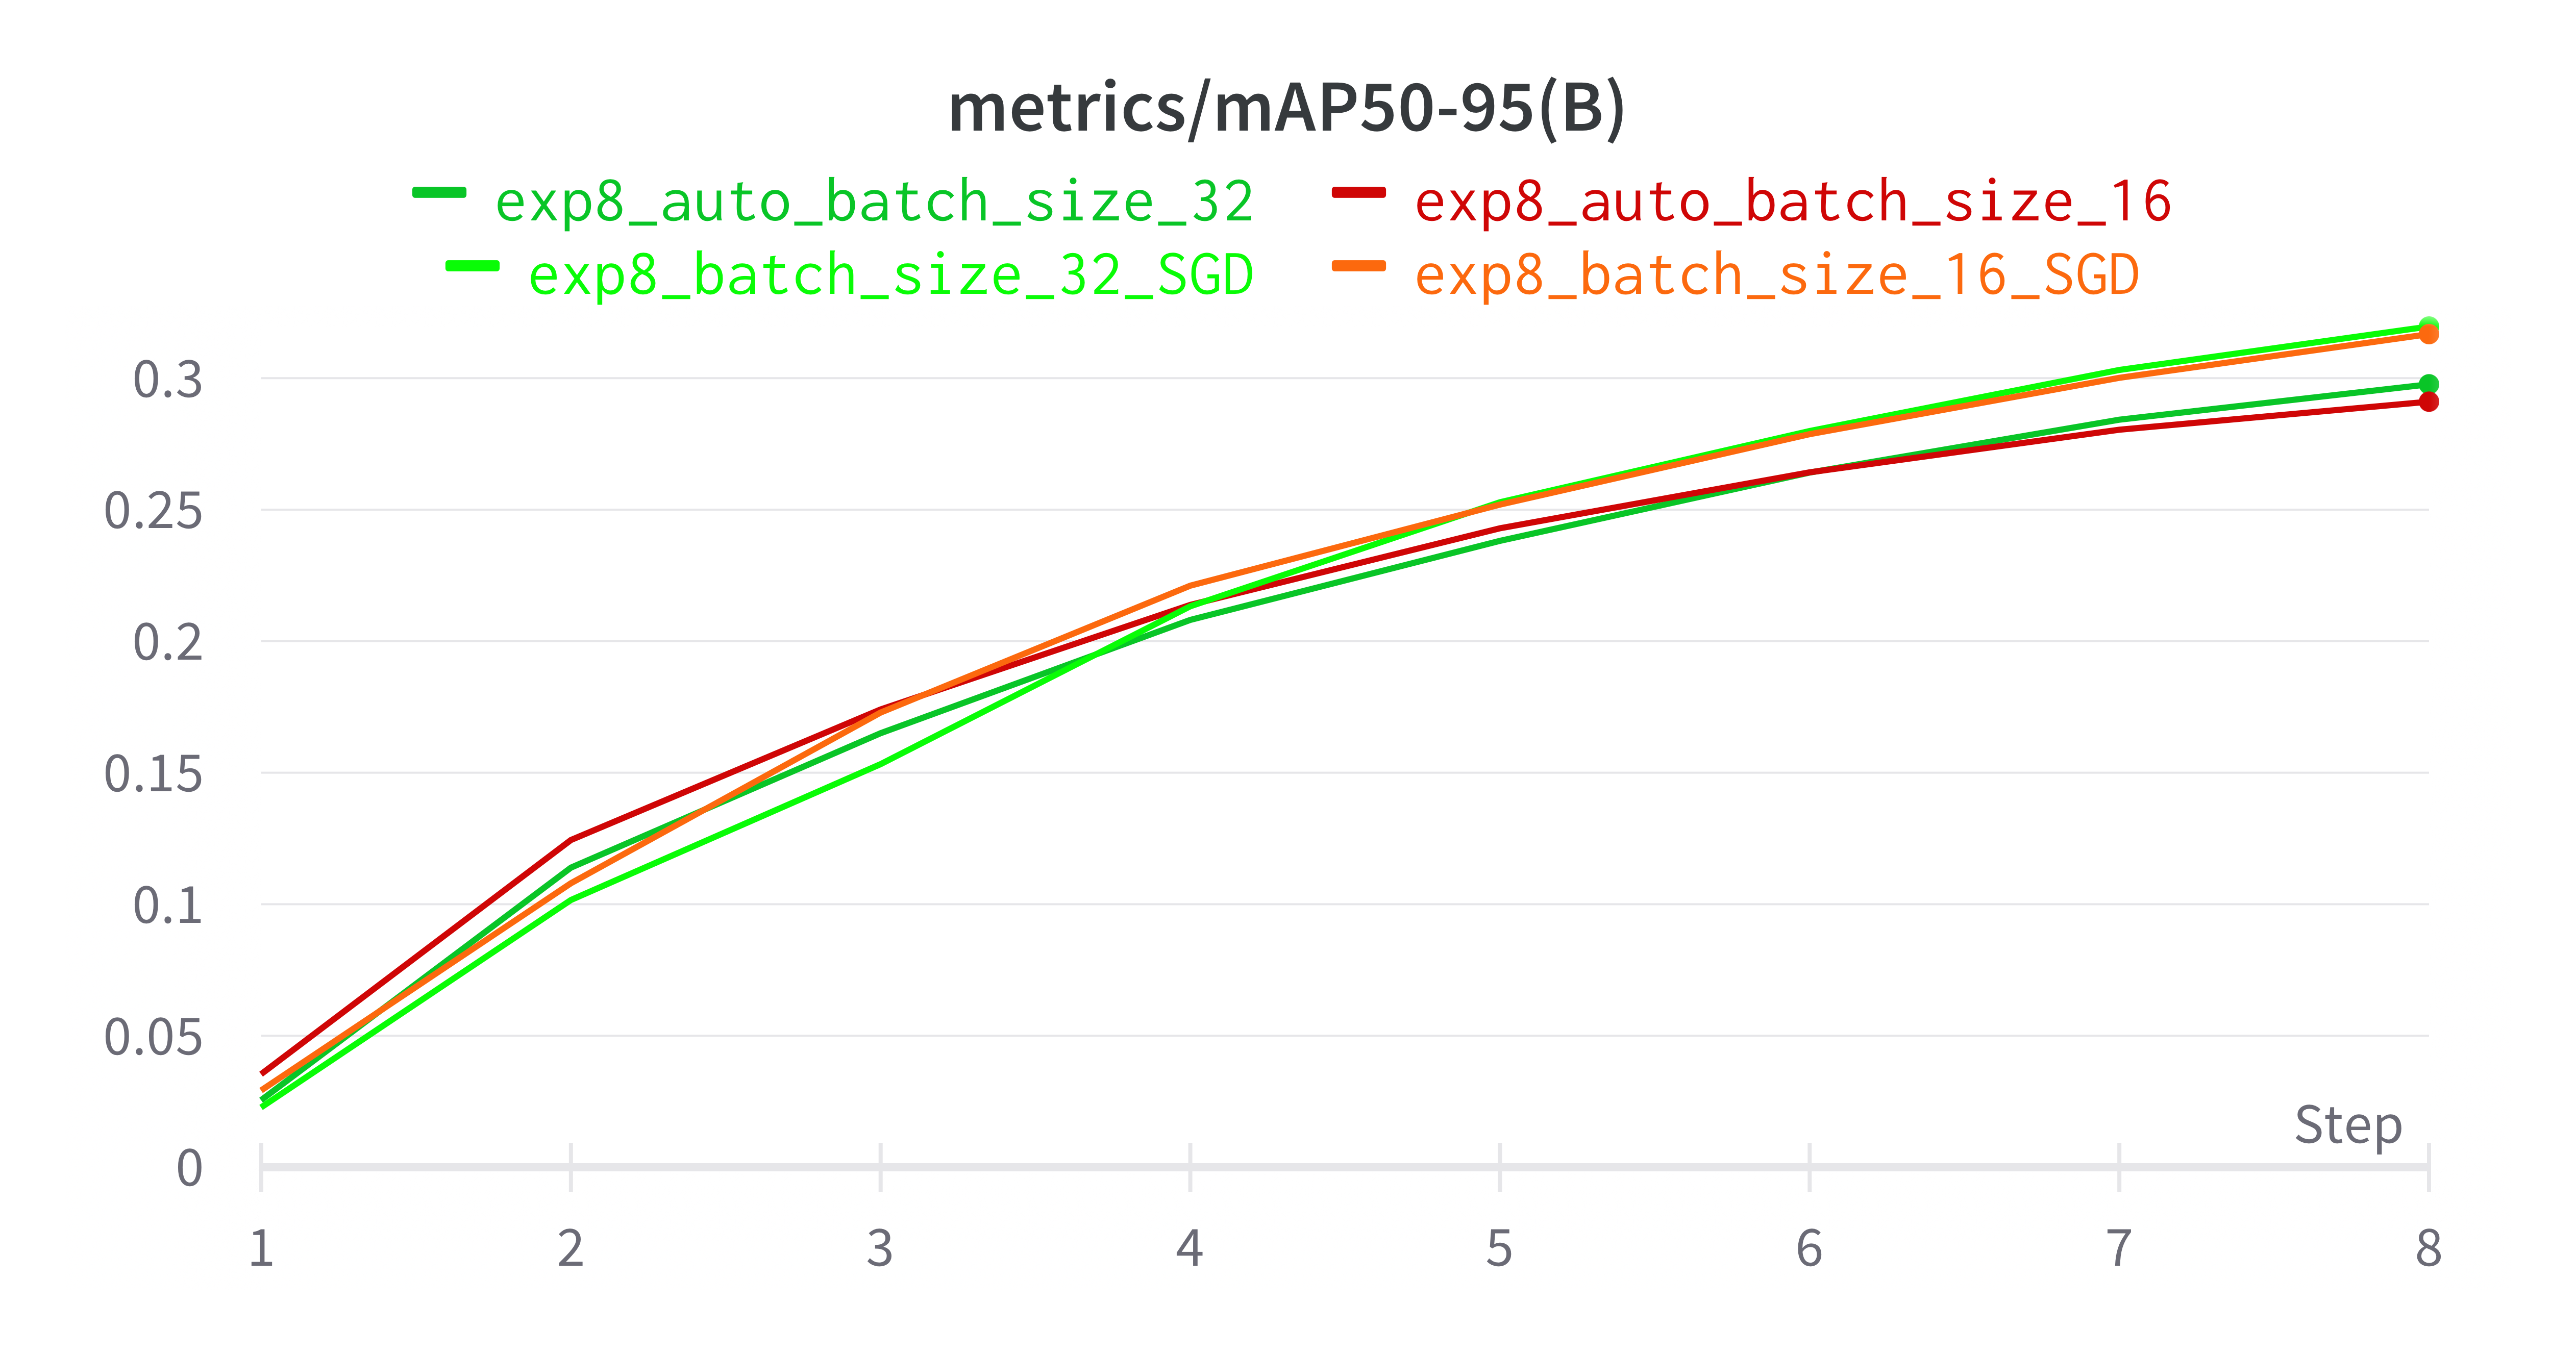
\includegraphics[width=0.4\textwidth,keepaspectratio]{mAP_batch_size_comparison.png} % TODO ; change file name
\caption{Comparison of mAP50-95 between training the model using batch size 16 and 32}
\label{fig:batch_size}
\end{figure}

\begin{figure}[h!]
\centering
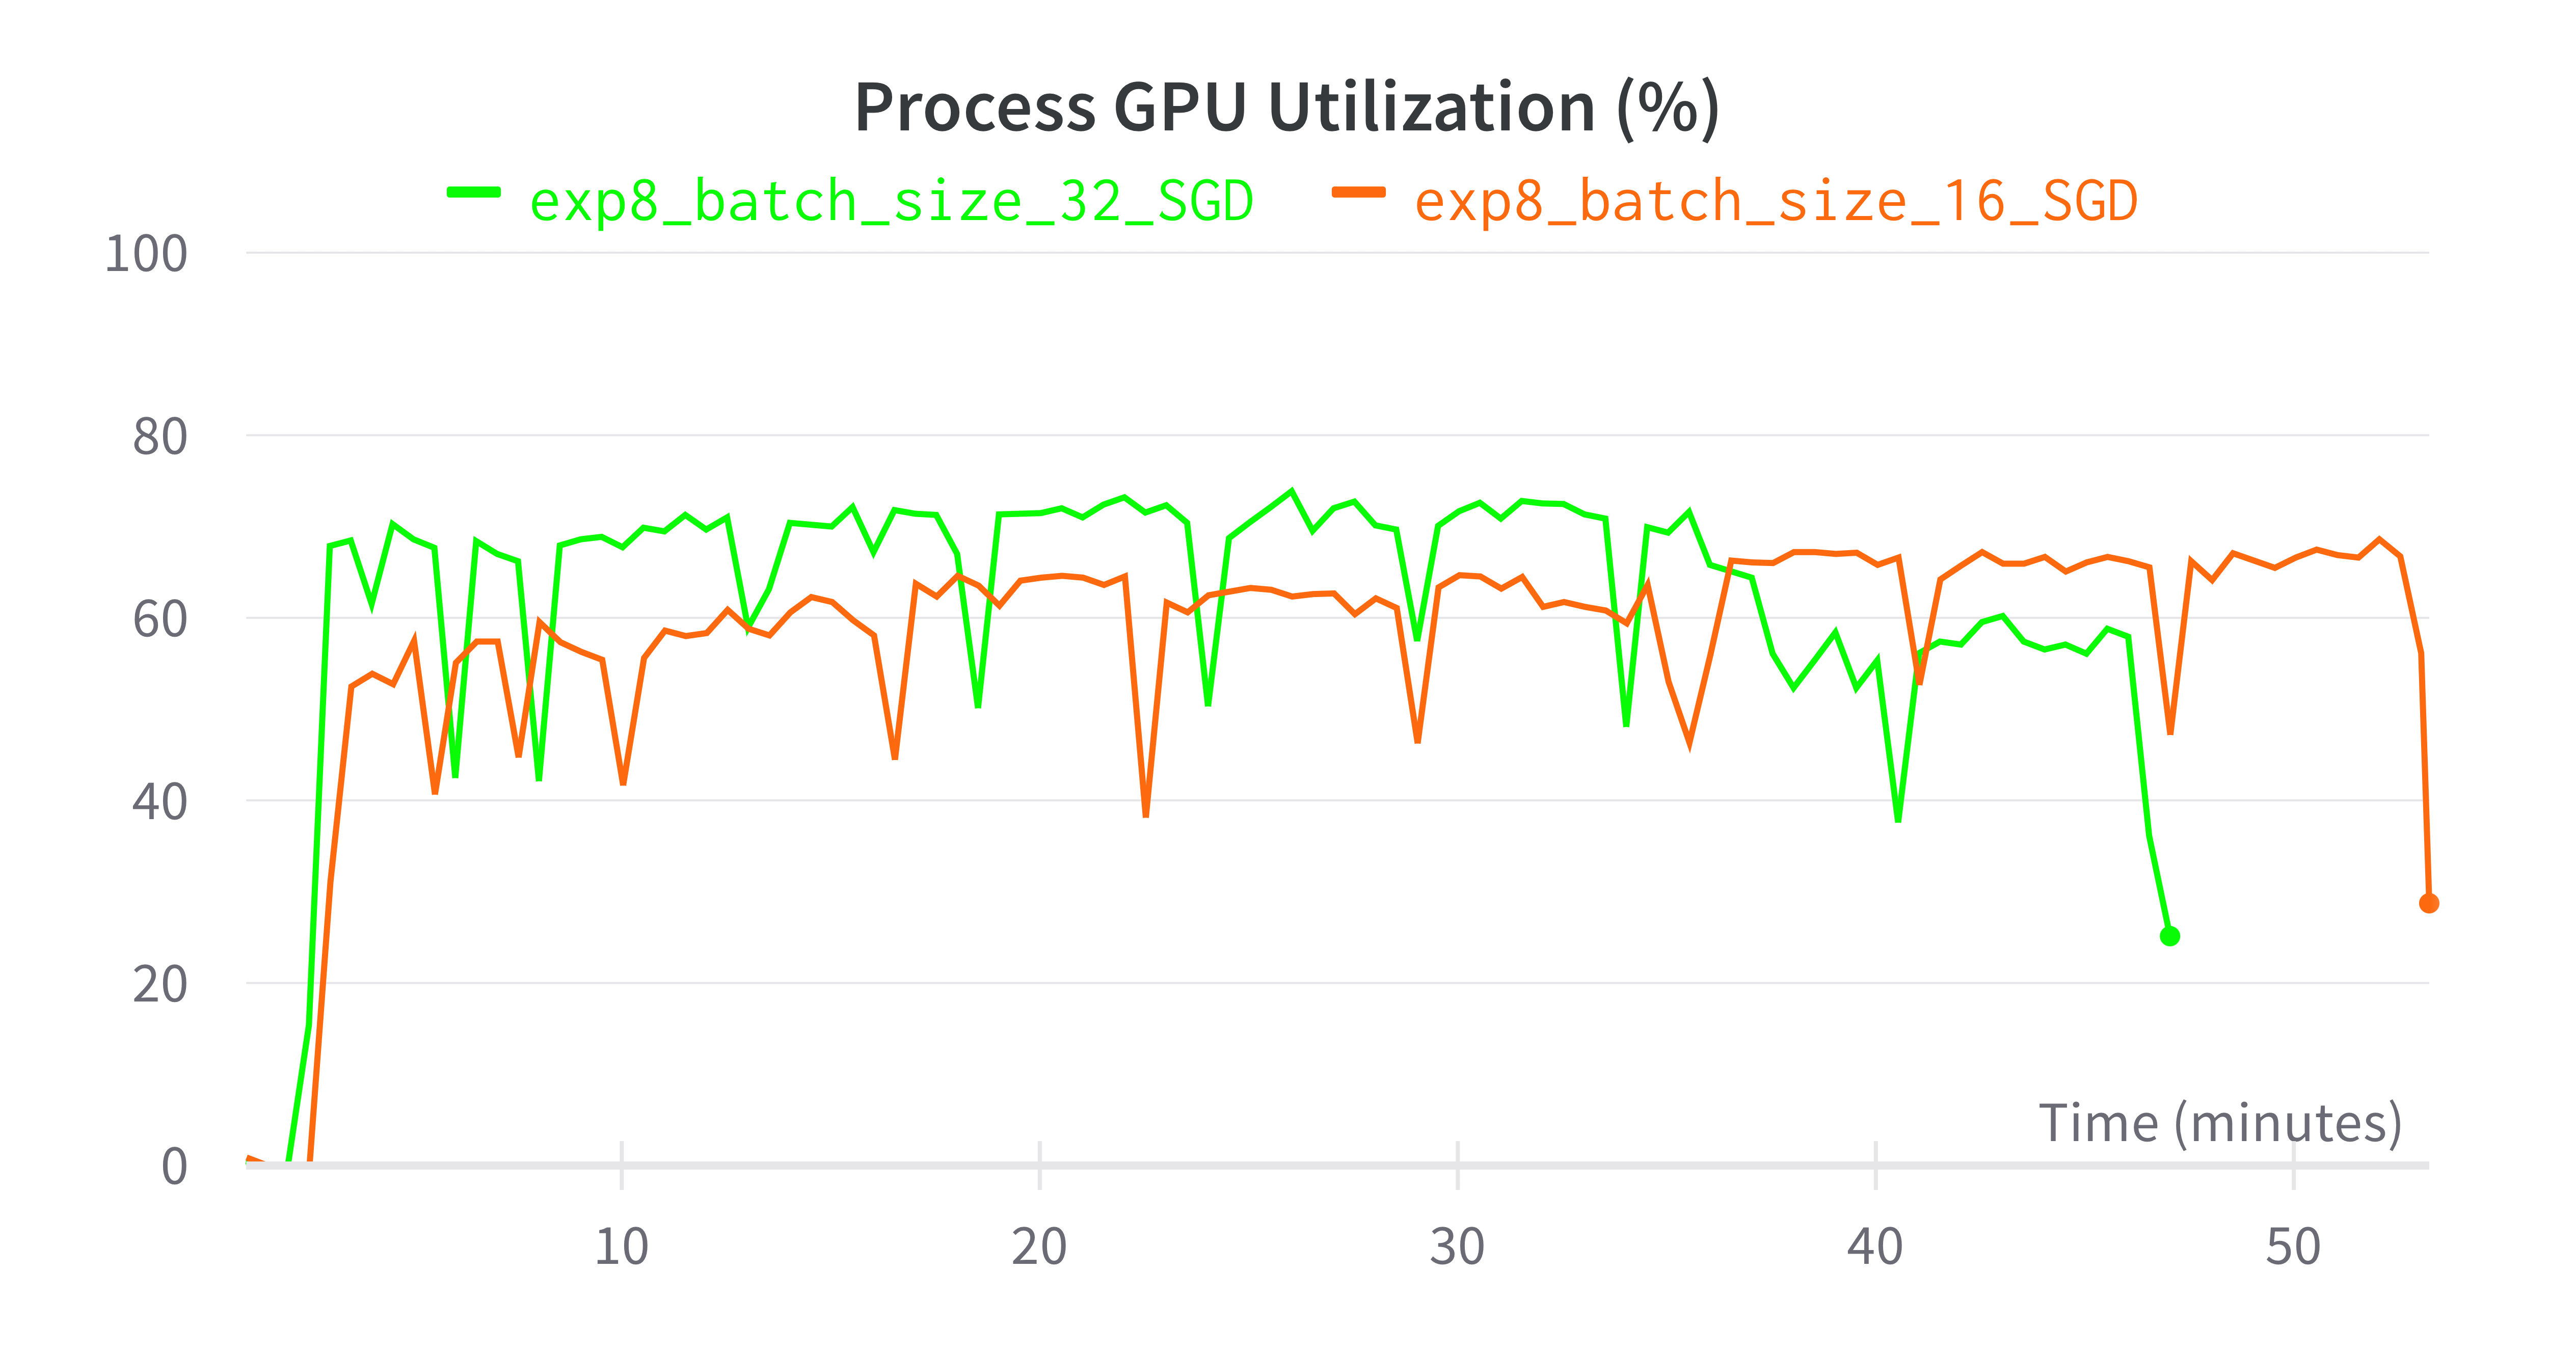
\includegraphics[width=0.4\textwidth,keepaspectratio]{gpu_utilization_comparison.png} 
\caption{Comparison of GPU Utilization between training the model using batch size 16 and 32}
\label{fig:gpu_utilization}
\end{figure}
% gpu_utilization_comparison.png
Fig.\ref{fig:batch_size} shows the result of training with different batch size. It can be observed that batch size 32 performs better than batch size 16. Especially in terms of training time, batch size 32 is faster than batch size 16.
Batch size 32 is employed for training purposes. Attempts were made to utilize both SGD and Adam optimizers. YOLOv8 implements optimizer switching depending on the number of iterations.


\subsection{Real World Testing}
In this section, we will discuss real-world testing. We bring the system to real-world environment scenario, placed our whole system into the dashboard of vehicles.
\begin{figure}[h!]
\centering
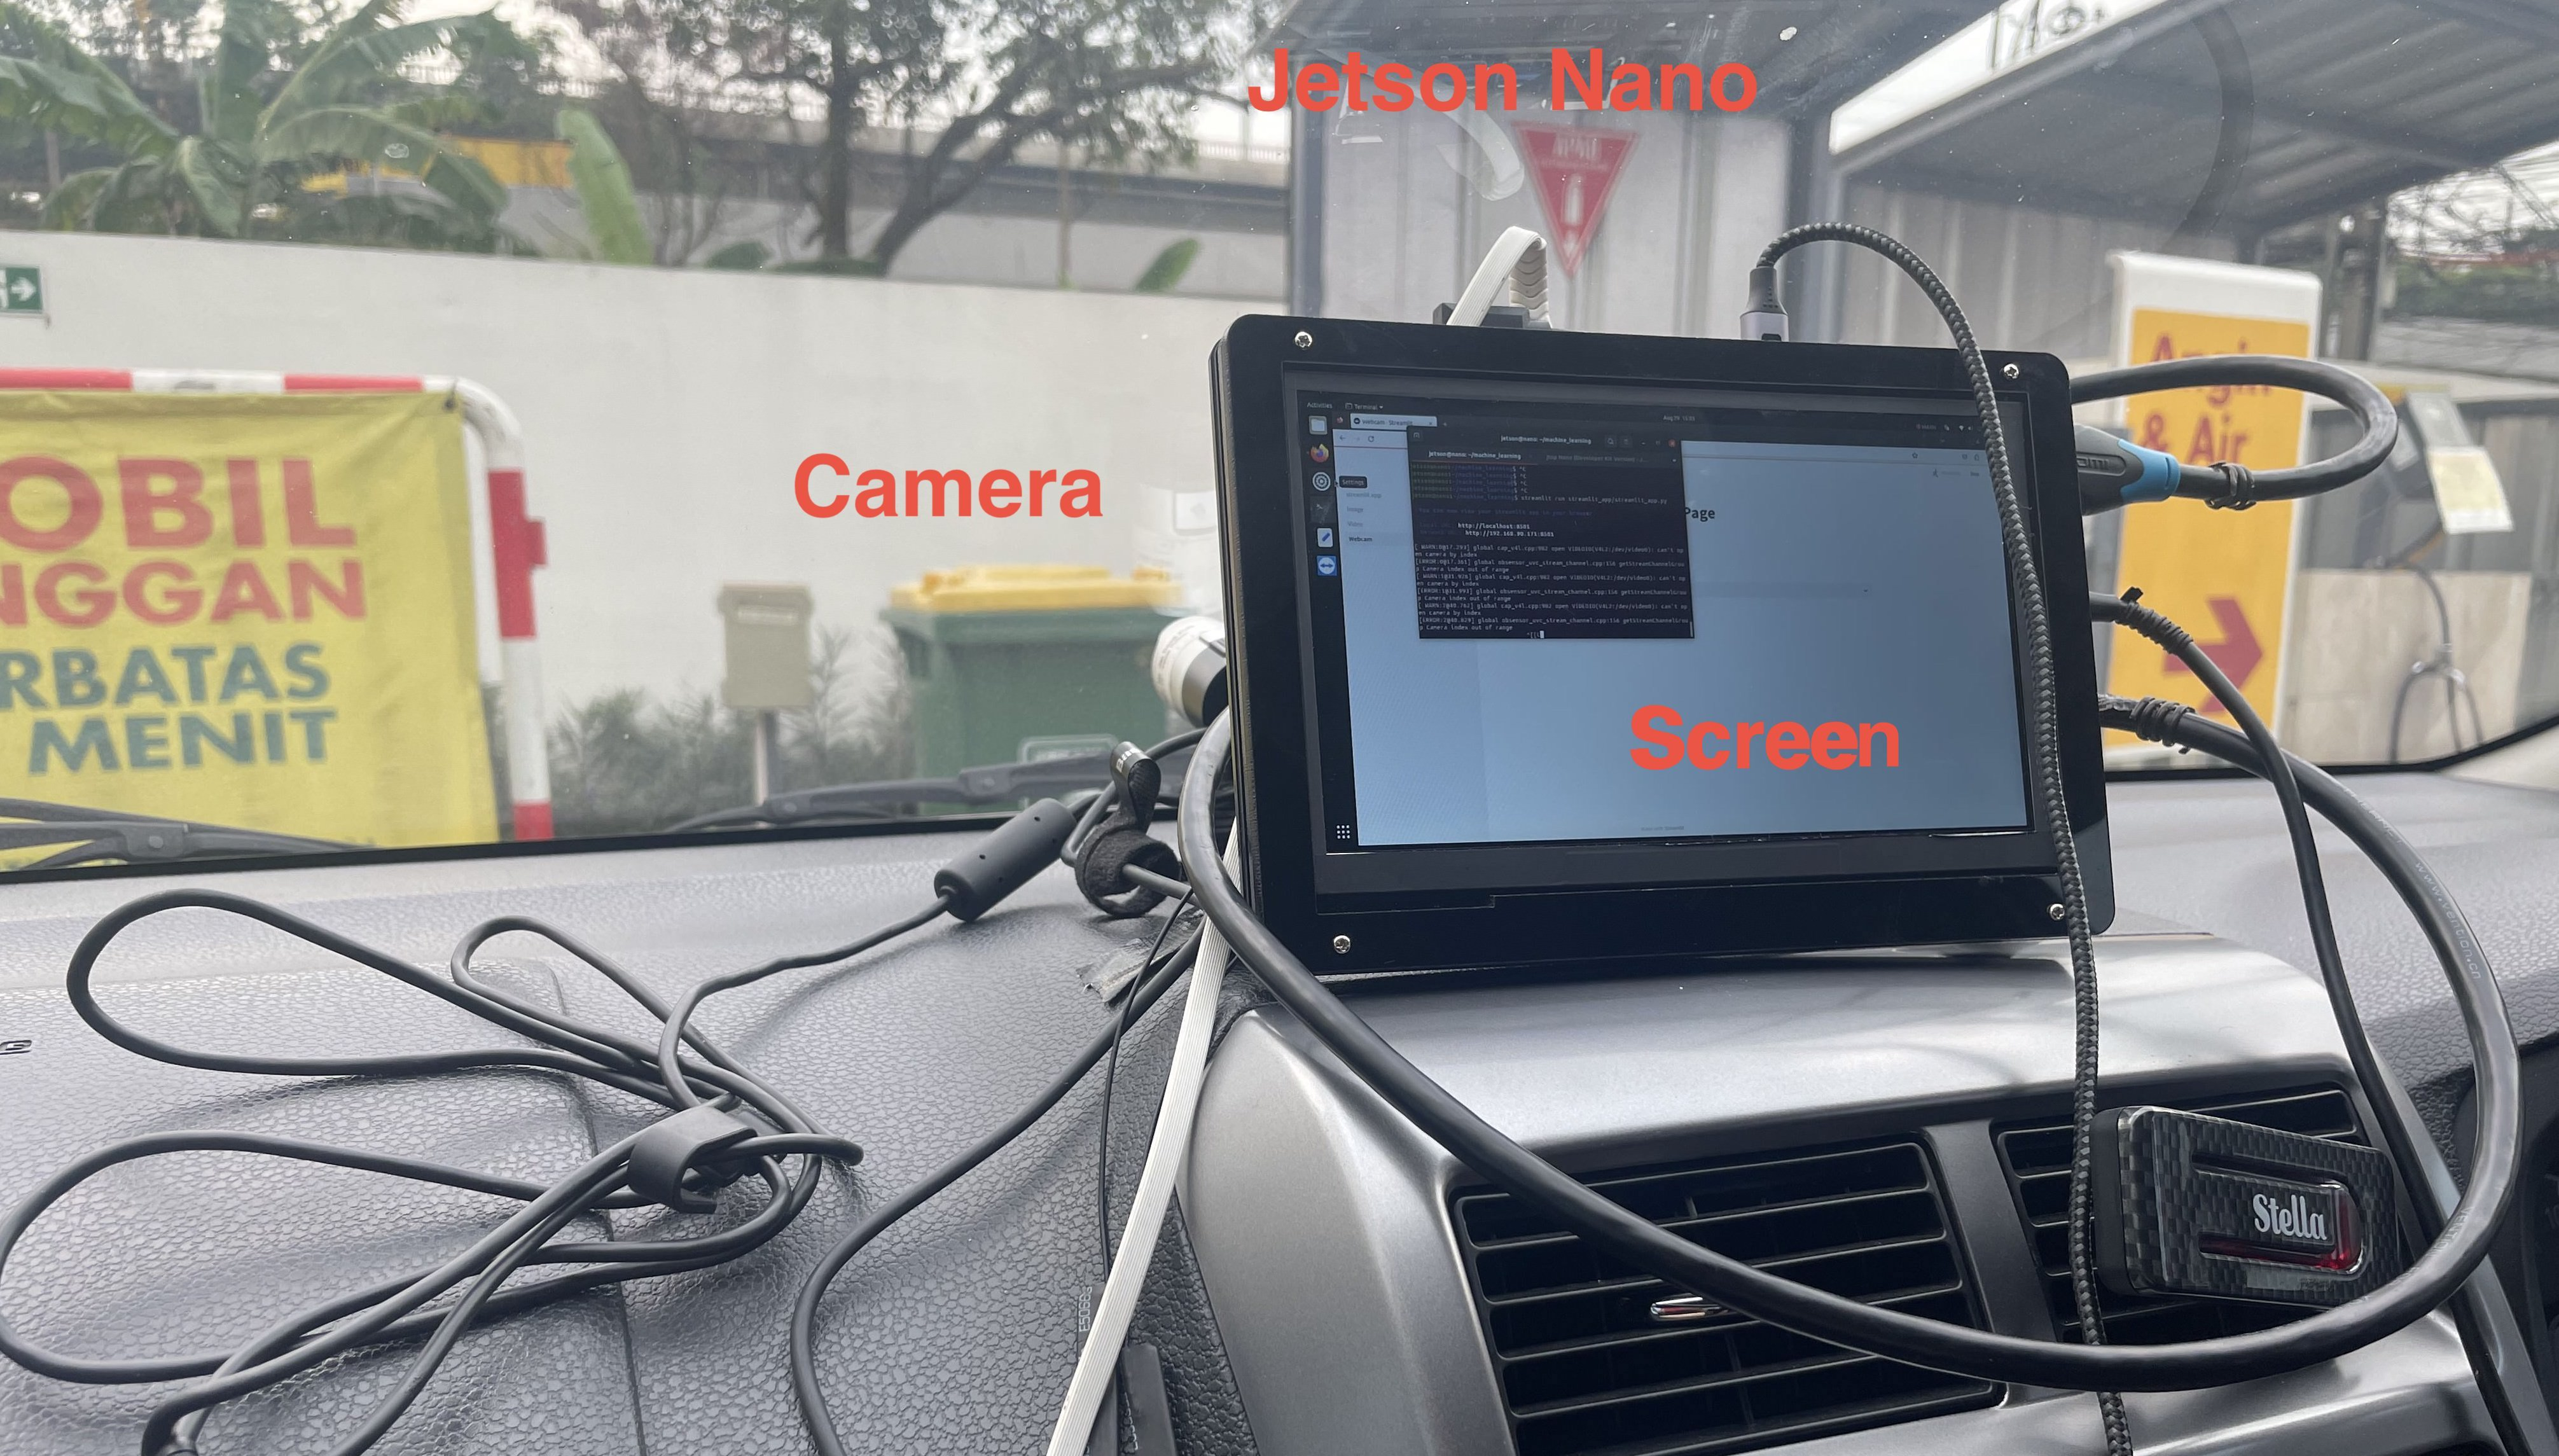
\includegraphics[width=0.4\textwidth,keepaspectratio]{mounted_camera_front_view.jpg}
\caption{Front View}
\label{fig:front_view}
\end{figure}

\begin{figure}[h!]
\centering
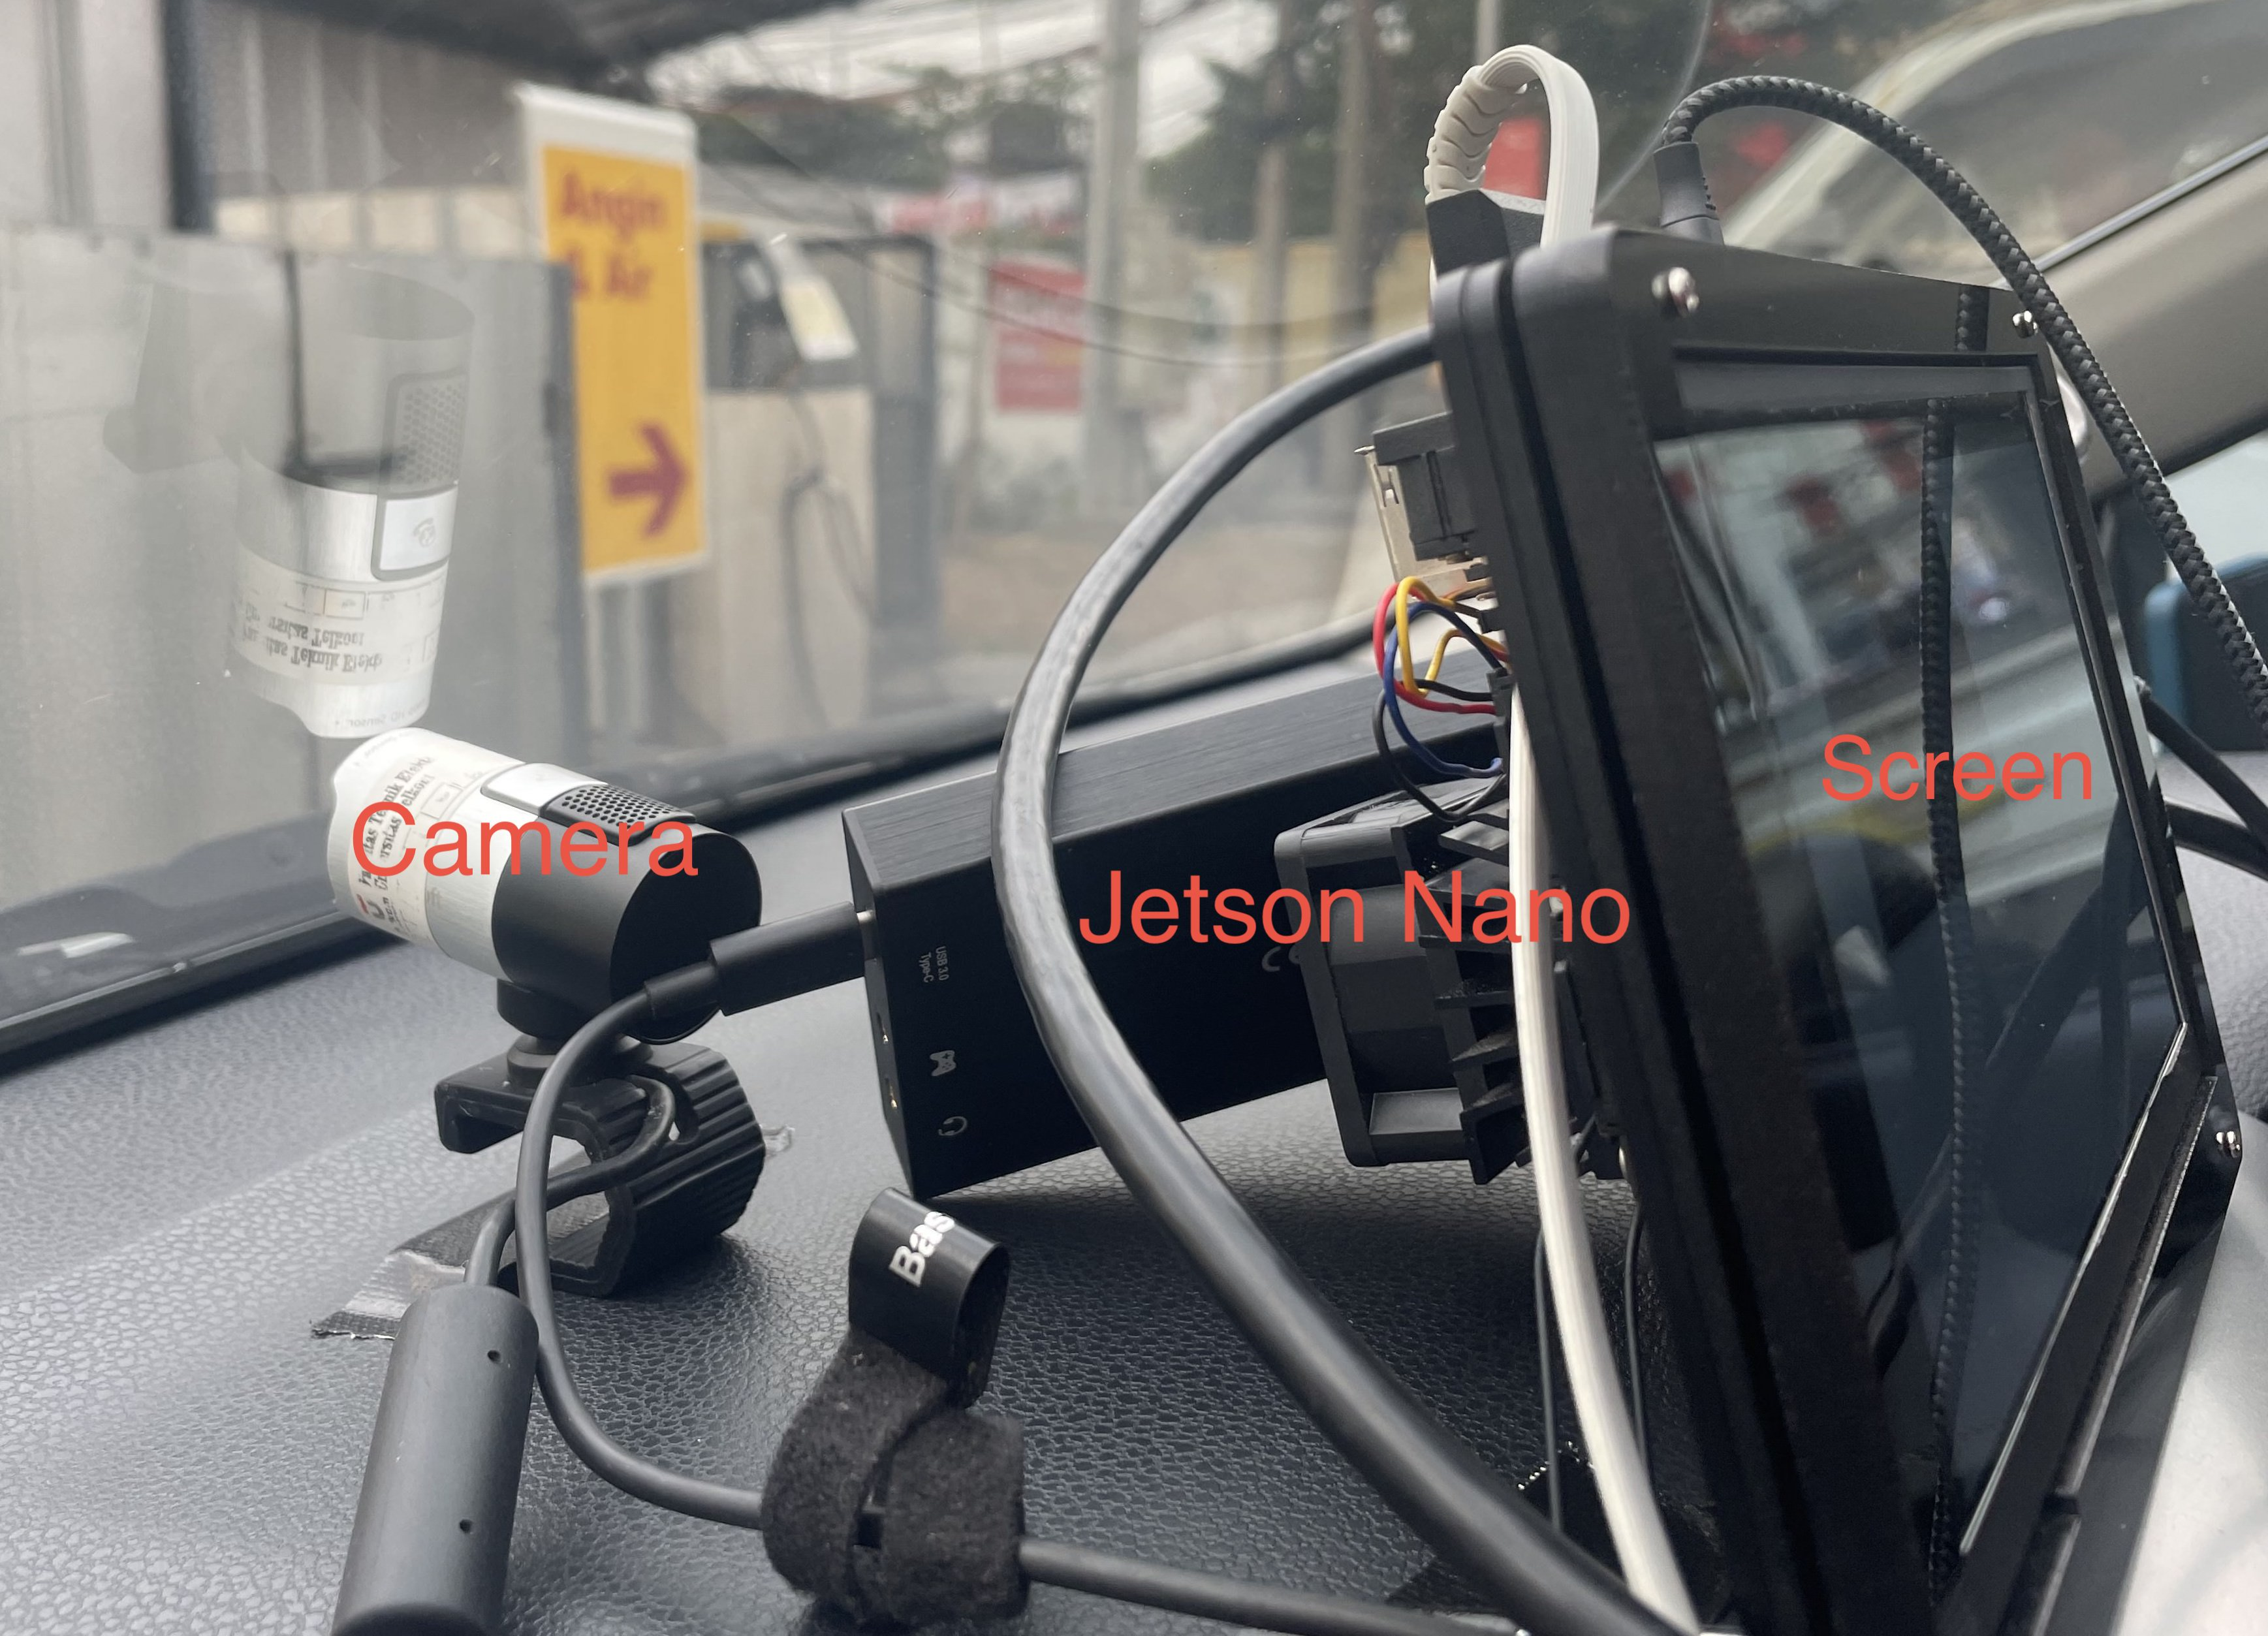
\includegraphics[width=0.4\textwidth,keepaspectratio]{mounted_camera_side_view.jpg}
\caption{Side View}
\label{fig:side_view}
\end{figure}
We use a USB car charger to power the whole system. We drove around the city of Bandung to test the system. 

\section{Results and Discussion}
In this section, we will discuss the result of our experiment. We will discuss the results of training and real-world testing.
\subsection{Training Result}
In this section, we will discuss the result of our object detection model training. We use the configuration concluded from the previous section. First, train the model with 80 epochs.
Then, in order to compare the performance of YOLOv8n model, we also train YOLOv7-tiny model.
Similar to YOLOv8n being the smallest model in the YOLOv8 series, YOLOv7-tiny is also the smallest model in the YOLOv7 series However, it needs more computation power than YOLOv8n. We train both YOLOv7-tiny and YOLOv8n with 80 epochs.
Fig.\ref{fig:mAP_comparison} indicates that YOLOv7-tiny is slightly better than YOLOv8n in terms of mAP50-95. However, YOLOv8n is better than YOLOv7-tiny.
\begin{figure}

\centering
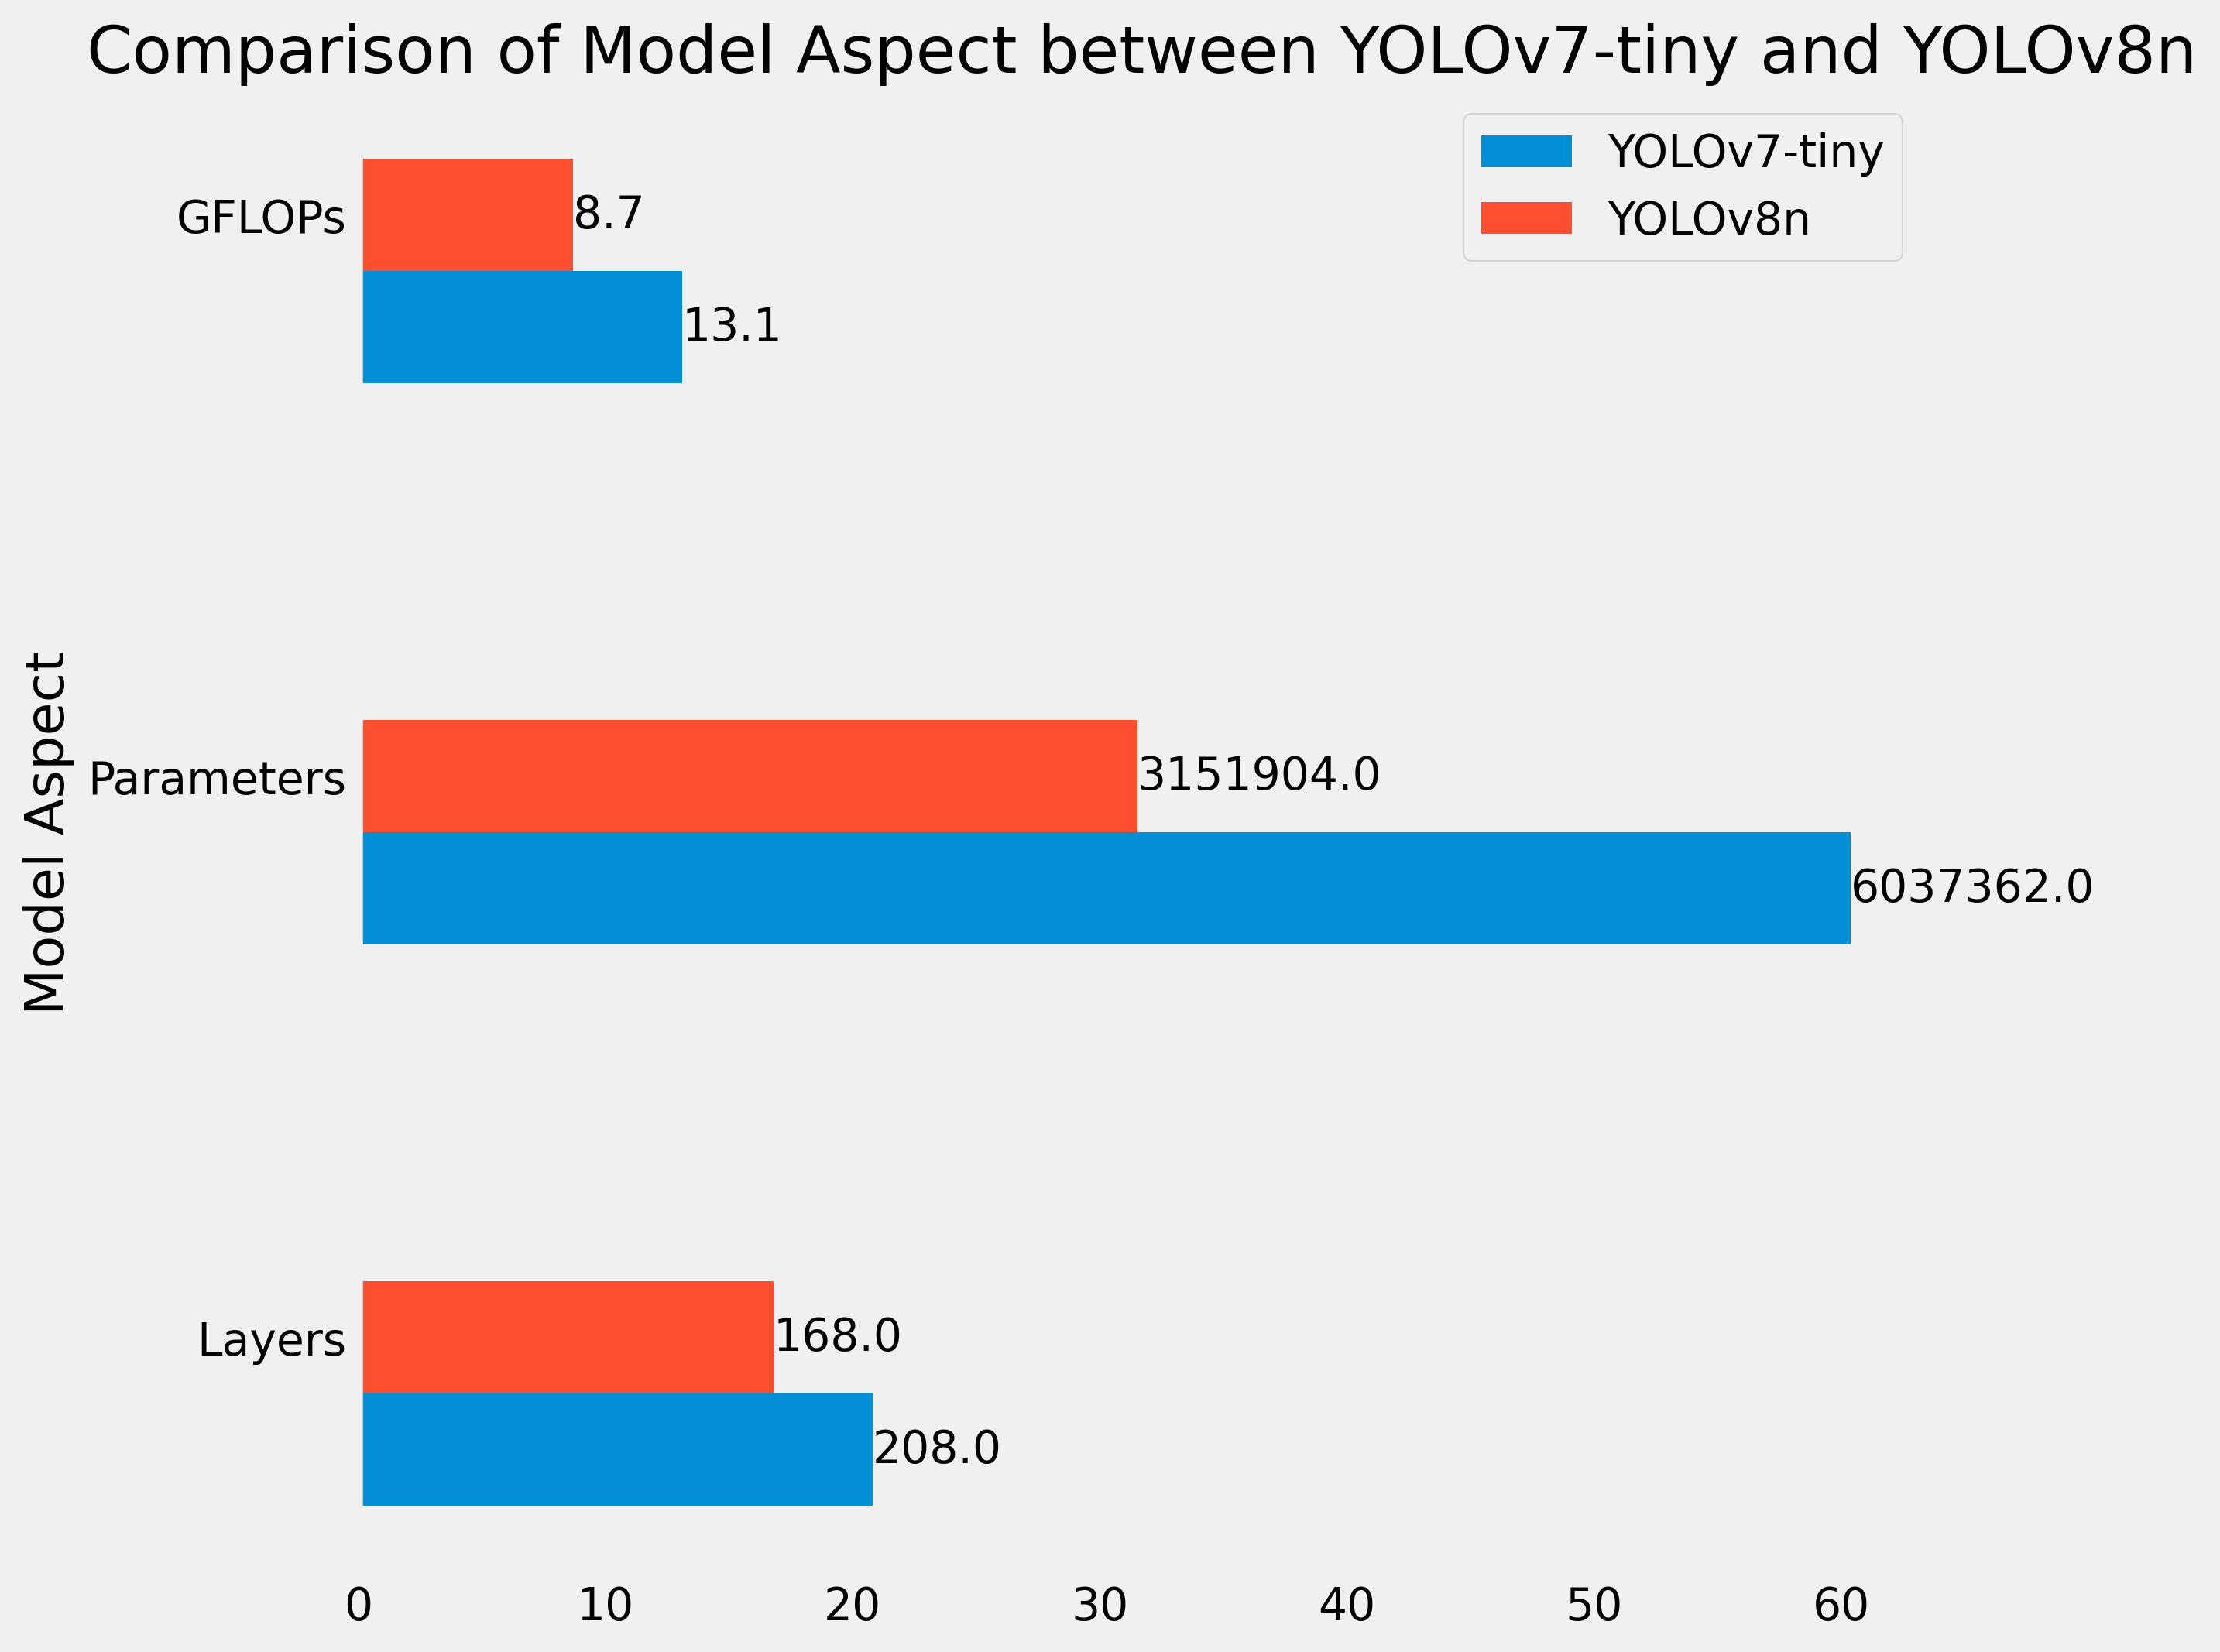
\includegraphics[width=0.4\textwidth,keepaspectratio]{YOLOv7-tinyvsYOLOv8n_model_aspect.png}    
\caption{Layers, Parameters, and GFLOPs Comparison between YOLOv7-tiny and YOLOv8n}
\end{figure}

\begin{figure}[h]
\centering
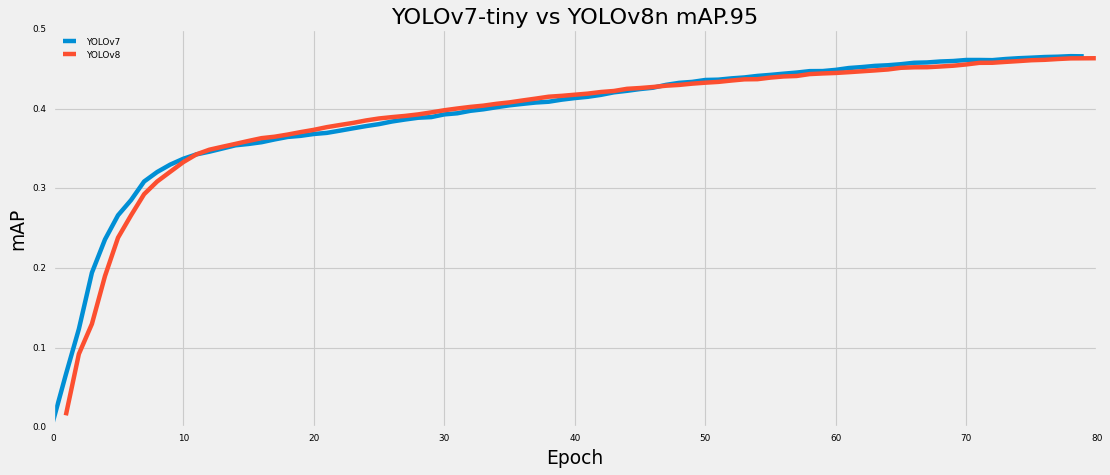
\includegraphics[width=0.4\textwidth,keepaspectratio]{YOLOv7-tinyvsYOLOv8n.png}
\caption{Comparison of mAP50-95 between YOLOv8n and YOLOv7-tiny}
\label{fig:mAP_comparison}
\end{figure}


We aim to run the model on an edge computer in real-time, so we must consider the inference time. As mentioned earlier, the computational cost of YOLOv8n is 8 GFLOPs while YOLOv7-tiny is 13 GFLOPs.
YOLOv8n is preferred due to its lower computational cost. Therefore, to achieve the performance level of YOLOv7-tiny, an attempt is made to train YOLOv8n for a more significant number of epochs. Twenty epochs were then added to the training process. YOLOv8n is trained for 100 epochs this time. Fig.\ref{fig:YOLOv7vsYOLOv8,80,100} shows the comparison of results between YOLOv7-tiny, YOLOv8n with 80 epochs, and YOLOv8n with 100 epochs.
\begin{figure}[h!]
\centering
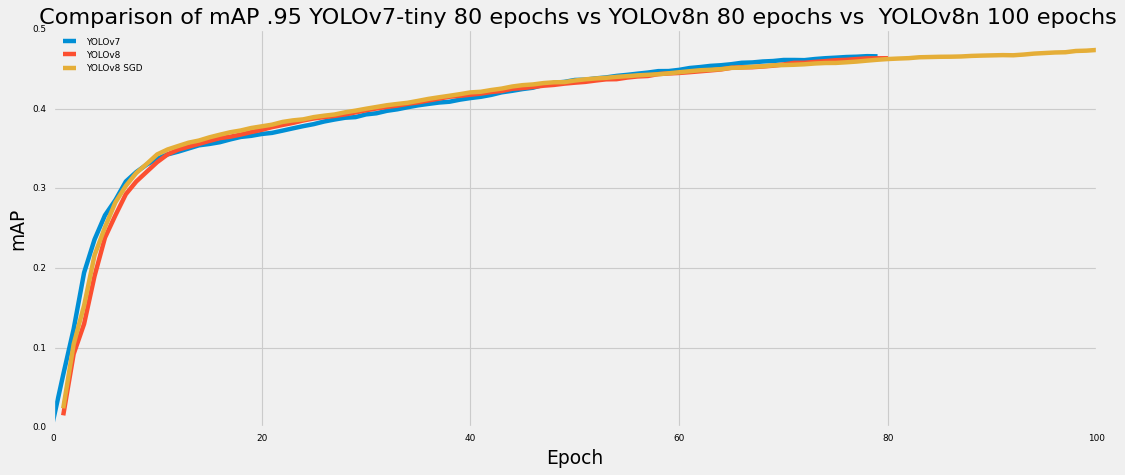
\includegraphics[width=0.4\textwidth,keepaspectratio]{YOLOv7vs YOLOv8,80,100.png}
\caption{Comparison of mAP50-95 between YOLOv7-tiny, YOLOv8n with 80 epochs, and YOLOv8n with 100 epochs}
\label{fig:YOLOv7vsYOLOv8,80,100}
\end{figure}
Finally, with 100 epochs training, the YOLOv8n model achieves similar metrics results with YOLOv7-tiny, despite being lower in computation cost.

\subsection{Real-World Testing Result}
The test result shows that the system can detect traffic objects in a real-world environment. Earlier, it was mentioned that a car charger is used to power the system. While the system is running, the other port on the same car charger is utilized for charging a smartphone. This results in different power available for the system. By doing this, it simulates real user scenarios. In a user scenario, the user might use the other port on the car charger to charge their smartphone. Many cars only have one port for a car charger and no other USB power inside the car. As a result, the system can run in 3 different power consumption. 5 Watt, 7 Watt, and 10 Watt.

\begin{equation}\label{FPS}
    Frame Per Second = \frac{1000}{latency}
\end{equation}

\begin{figure}[h!]
\centering
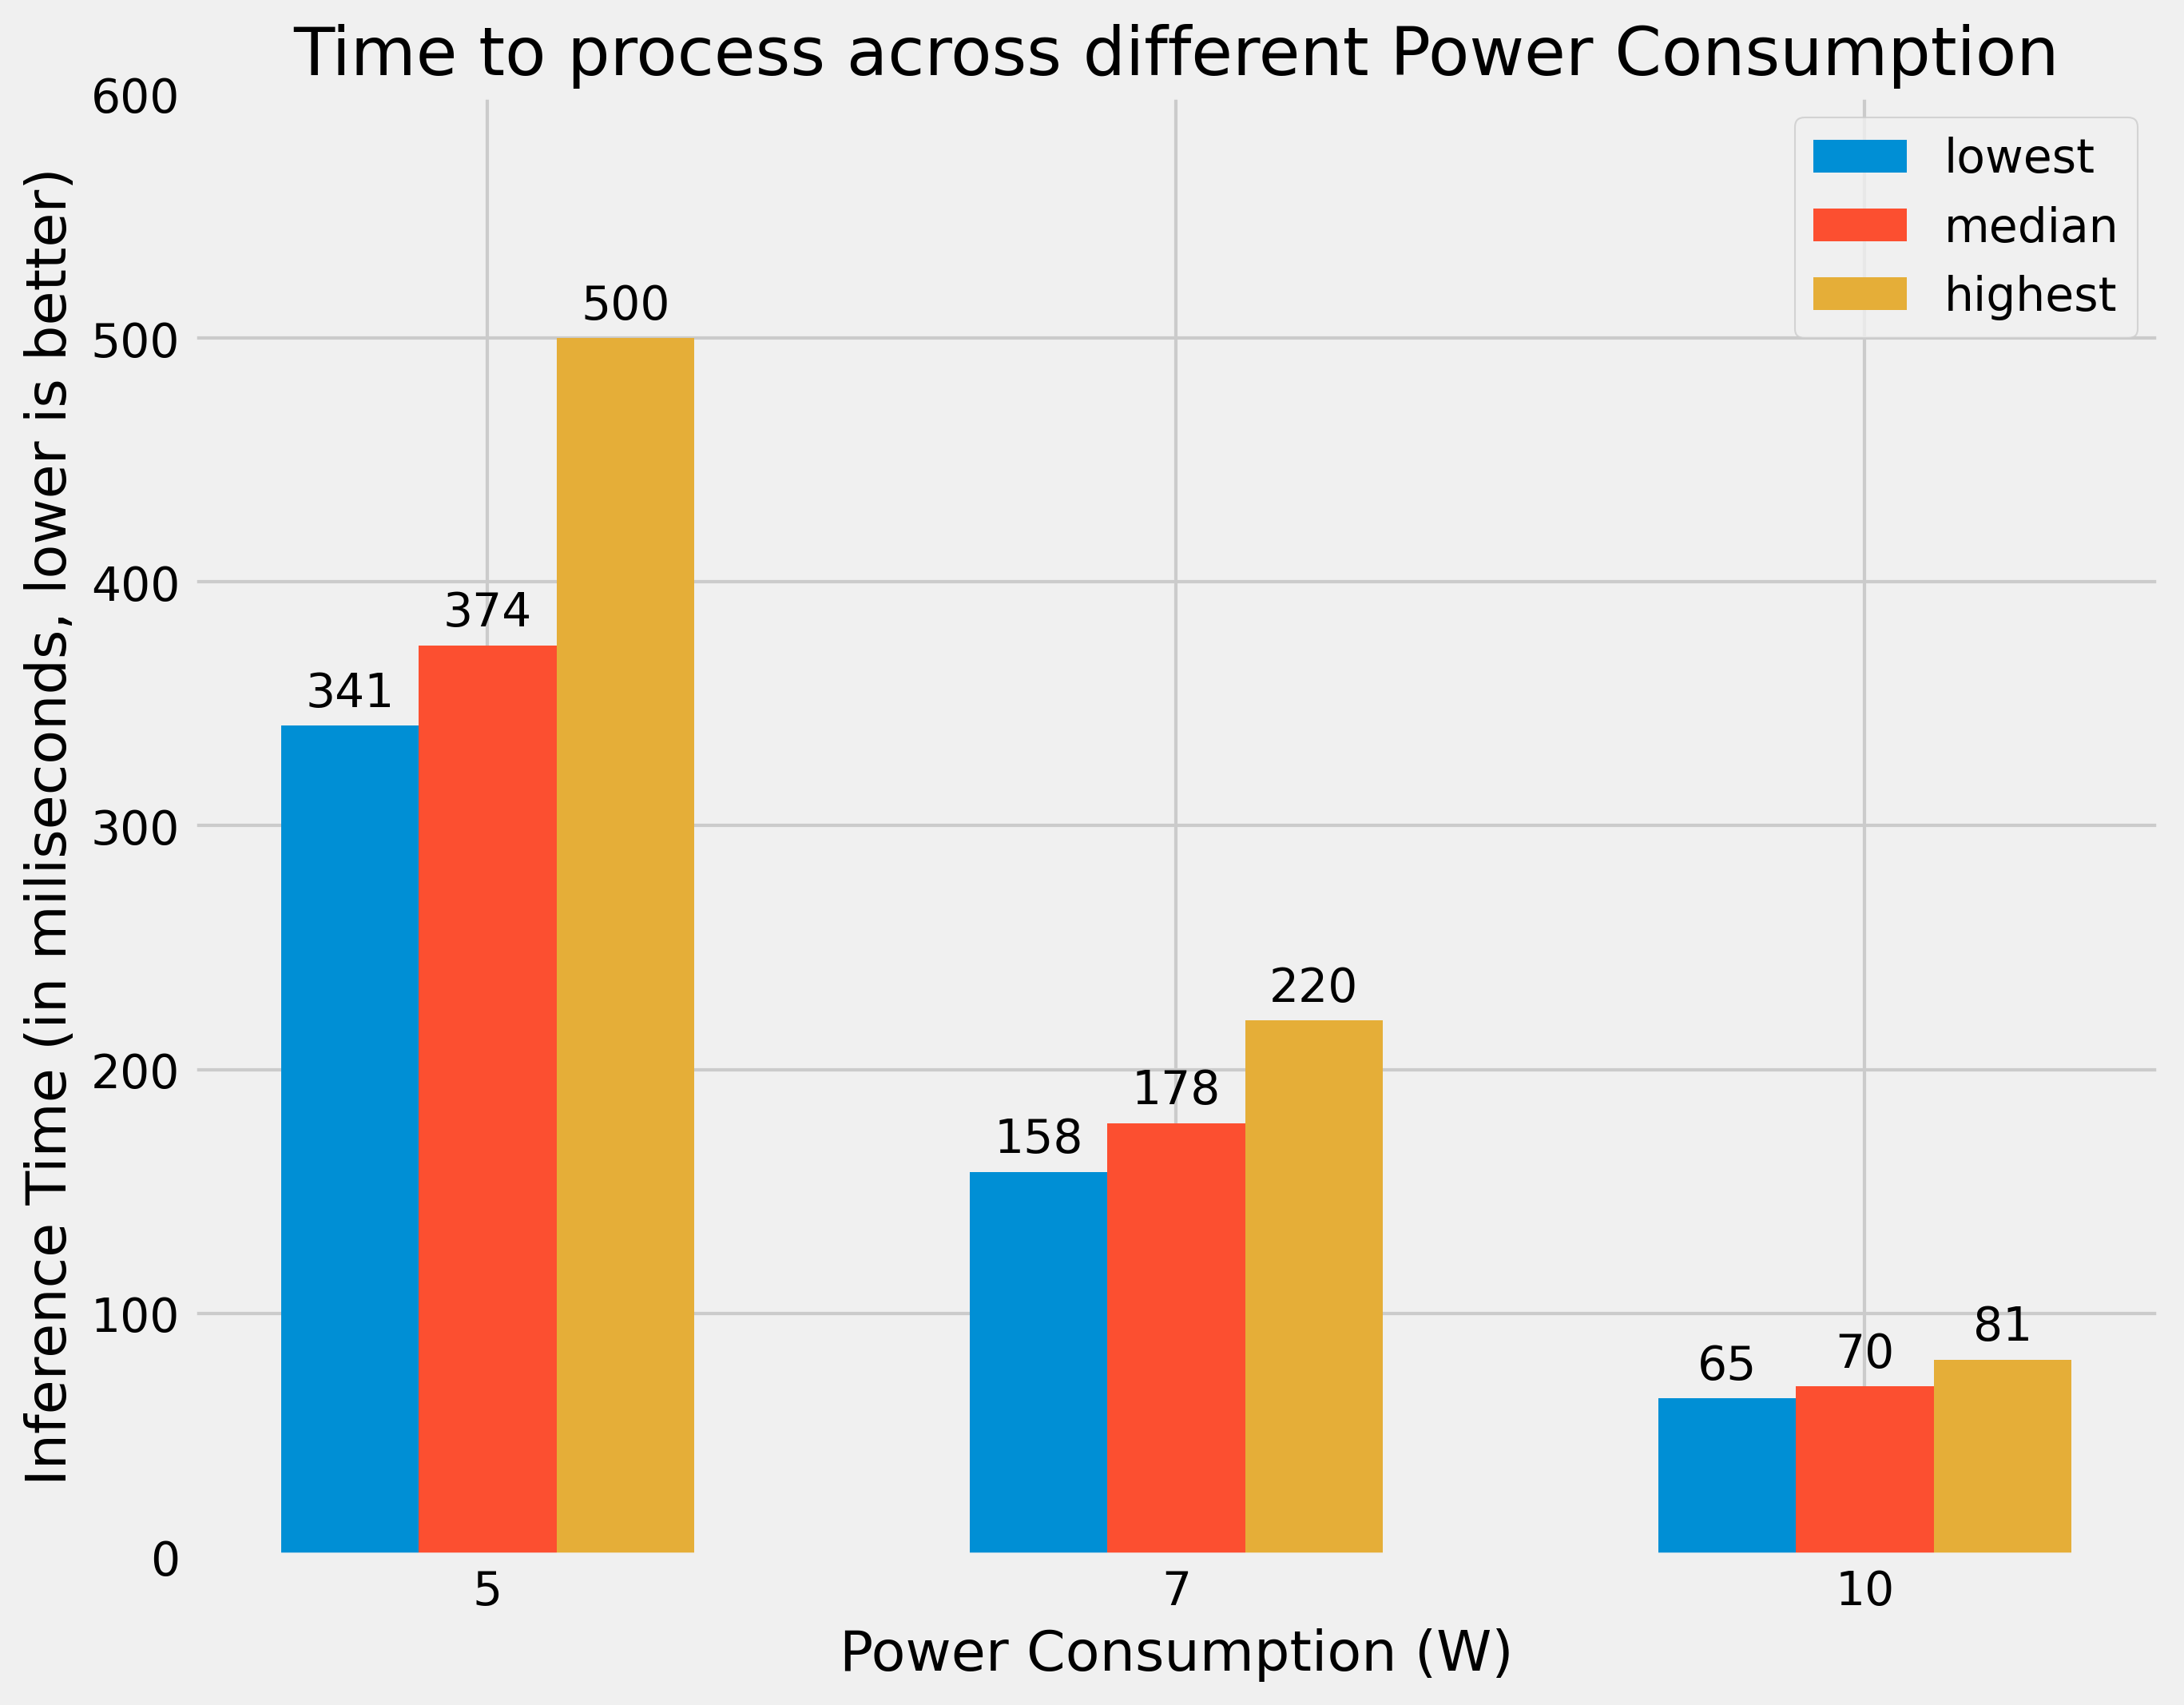
\includegraphics[width=0.4\textwidth,keepaspectratio]{inference_time_comparison.png}
\caption{Inference Time Comparison across different Power Consumption, Power Consumption error range is within 1 Watt}
\label{fig:inference_time_comparison}
\end{figure}
The motorcycle and its rider were found to be the most challenging traffic object to detect. At the same time, some random red or green lights can be detected as traffic lights.
On the other hand, the system can detect Car 90\% of the time.

In terms of inference time, we gather the data by running the system in 3 different power consumption. 5 Watt, 7 Watt, and 10 Watt. We record the inference time data in miliseconds.
We record the inference time data in milliseconds. Many researchers use FPS (Frame Per Second) as their metric for inference. We can convert inference time into FPS by using Eq~\eqref{FPS}

Based on Eq \eqref{FPS} and Fig.\ref{fig:inference_time_comparison}, we can conclude that FPS and inference time are inversely proportional. As the inference time increases, the FPS decreases. If we want smoother video output, we need to increase the FPS. In other words, we must reduce the inference time to get a smoother video output flow.\@.

\section{Conclusion}
Dashcam has become a popular device for drivers to record road condition. However, the dashcam video is not only used for recording the road condition, but also used for other purposes, such as insurance claims.
In this paper, we proposed a dashcam system to detect traffic objects. The object detection system is based on the YOLOv8n model. We also proposed a dataset for dashcam traffic object detection. The dataset was created by filtering the MS COCO Dataset and adding our own annotated images. The dataset contains 78000 images with 12 traffic objects class.
The training time can be reduced and the model performance is increased by filtering the dataset.
We also propose a dashcam system that can be used for testing. The system is built using Jetson Nano 4GB as the edge computer.


It can be concluded that system can detect traffic objects in a real-world environment based on the results of the Real World Testing. Inference Time shows different results across different power consumption.
The system's power draw depends on the electrical power available in the vehicle. The result of inference time was obtained in 3 different power consumptions, namely 5, 7, and 10 Watt. With this power consumption, the system can do the inference under
90 milliseconds for an image size of 640 by 480. While in lower power consumption, 7 watts, the system can make the inference in around 150–220 milliseconds.
In 5-watt power consumption, the system can do the inference in around 340–500 milliseconds. If processing time were converted into Frames Per Second, it would result in a 2 to 15 FPS range. Based on the inference time and FPS results, we can conclude that the system can run in real-time while in 10-watt power consumption.
Although using Jetson Nano was sufficient to run the system, we need a higher-performance edge computer if we want to do further image processing and higher image resolution. Additional performance increases can be expected by using a more robust edge computer. Such as using newer hardware from the Nvidia Jetson Series. Further optimization can be done by using the full potential of GPU in the Nvidia Jetson Series.
Further optimization can be done by using the full potential of GPU in the Nvidia Jetson Series. Another alternative is rewriting or running inference in C++ instead of Python, as in this experiment, which might improve the system's performance.
Further development towards Autonomous Driving Assistance Systems (ADAS) can be done by collaborating more cameras and sensors.
% \section*{Acknowledgment}
% This research is supported by Telkom University, Indonesia.
% We would like to personally thank M Rayhan Aryana for his help in this research.
% Especially in the process of gathering the dataset and testing the system in   environment.
% We also would like to thank QEngineering for open-sourcing their Jetson Nano Ubuntu 20.04 image. With their Operating System image that was preinstalled with OpenCV and Pytorch, compiled with CUDA support, we can save a lot of time in setting up the environment.



\bibliographystyle{IEEEtran}
\begin{thebibliography}{00}
\bibitem[1]{b1} A. Soin and M. Chahande, “Moving Vehicle Detection Using Deep Neural Network.” A. Soin and M. Chahande, “Moving Vehicle Detection Using Deep Neural Network.” 
\bibitem[2]{Korea Dashcam} Kim, J., Park, S., and Lee, U. (2020). Dashcam Witness: Video Sharing Motives and Privacy Concerns Across Different Nations. IEEE Access, 8, 110425–110437. doi:10.1109/access.2020.3002079 
\bibitem[3]{Object Detection in 20 Years} Z. Zou, K. Chen, Z. Shi, Y. Guo, and J. Ye, “Object detection in 20 years: A survey,” Proceedings of the IEEE, vol. 111, no. 3, pp. 257–276, 2023. doi:10.1109/jproc.2023.3238524 
\bibitem[4]{b3} Krizhevsky, A., Sutskever, I., Hinton, G. E. (2012). ImageNet classification with deep convolutional neural networks. Communications of the ACM, 60(6), 84–90. https://doi.org/10.1145/3065386
\bibitem[5]{Rich feature hierarchies}J. Redmon, S. Divvala, R. Girshick and A. Farhadi, "You Only Look Once: Unified, Real-Time Object Detection," 2016 IEEE Conference on Computer Vision and Pattern Recognition (CVPR), Las Vegas, NV, USA, 2016, pp. 779-788, doi: 10.1109/CVPR.2016.91.
\bibitem[6]{You Only Look Once}J. Redmon, S. Divvala, R. Girshick and A. Farhadi, "You Only Look Once: Unified, Real-Time Object Detection," 2016 IEEE Conference on Computer Vision and Pattern Recognition (CVPR), Las Vegas, NV, USA, 2016, pp. 779-788, doi: 10.1109/CVPR.2016.91.
\bibitem[7]{COCO Dataset} T.-Y. Lin et al., “Microsoft Coco: Common Objects in Context,” Computer Vision – ECCV 2014, pp. 740–755, 2014. doi:10.1007/978-3-319-10602-1-48
\bibitem[8]{YOLO with adaptive frame} J. Lee and K. Hwang, “Yolo with adaptive frame control for real-time object detection applications,” Multimedia Tools and Applications, vol. 81, no. 25, pp. 36375–36396, 2021. doi:10.1007/s11042-021-11480-0
\bibitem[9]{Road Information Collector} S. M. Nasution, E. Husni, K. Kuspriyanto, R. Yusuf, and R. Mulyawan, “Road information collector using smartphone for measuring road width based on object and Lane Detection,” International Journal of Interactive Mobile Technologies (iJIM), vol. 14, no. 02, p. 42, 2020. doi:10.3991/ijim.v14i02.11530 
\bibitem[10]{YOLOv5 ADAS} S. M. Nasution and F. M. Dirgantara, “Pedestrian Detection System using Yolov5 for advanced driver assistance system (ADAS),” Jurnal RESTI (Rekayasa Sistem dan Teknologi Informasi), vol. 7, no. 3, pp. 715–721, Jun. 2023. doi:10.29207/resti.v7i3.4884 
\end{thebibliography}
\vspace{12pt}
\color{red}


\end{document}